\chapter{Quantum mechanics on a computer}

This chapter comprises a summary of some of the methods used by cold atom physicists to compute numerical results pertaining to cold atom systems. Many a problem in quantum mechanics is not analytically solvable, especially when the real world of experimental physics rears its ugly head, violating theorists' assumptions of simplicity left and right. In particular, atomic physics experiments are time-dependent, with each run of an experiment generally proceeding in stages. Lasers may turn on and off, magnetic fields may vary in magnitude and direction, \textsc{rf} pulses may be chirped to reliably induce particular transitions \cite{bennie_precise_2014}. Much of the numerical computation performed by researchers in cold atom physics groups such as ours are accordingly of the time-dependent variety, and are fairly literal simulations of specific experiments that may be carried out in the lab.

Here I explain some fundamentals of representing quantum mechanical problems on a computer and then present my favourite algorithms for propagating state vectors and wavefunctions in time. To spoil the surprise: my favourite timestepping algorithms are the 4th-order split-step method and (unoriginally) 4th-order Runge--Kutta, and my favourite method of evaluating spatial derivatives is moderate (6th or so) order finite differences. I think Fourier transforms for spatial derivatives are overrated, and I show that the finite element discrete variable representation (\textsc{fedvr}) is, despite appearances, actually less computationally efficient than simple finite differences for producing equally accurate solutions to the spatial Scr\"odinger equation. I also mention some methods of finding groundstates and other stationary states, and in section \ref{sec:rk4ilip} I present a modification to 4th-order Runge--Kutta that enables it to take larger timesteps for certain problems.

\section{From the abstract to the concrete: neglect, discretisation and representation}\label{sec:neglect_discretisation}

To numerically simulate a quantum mechanical system, one must evolve a state vector in time according to the Schr\"odinger equation:
\begin{align}\label{eq:schrodinger_equation}
\ii\hbar\dv{t}\ket{\psi(t)} = \hat H (t) \ket{\psi(t)}.
\end{align}
To do this on a computer, one must first decide which degrees of freedom are to be simulated. We necessarily neglect many degrees of freedom as a matter of course; which ones can be neglected is warranted by the specific situation and we do it so often we barely notice. For example, simulating a single component Bose--Einstein condensate entails neglecting the internal degrees of freedom of the atoms---as well as reducing the atom-light interaction to a simple potential such as an optical dipole trap or magnetic dipole interaction (neglecting the quantum degrees of freedom in the electromagnetic field). We may ignore one or more spatial degrees of freedom as well, say, if we are simulating an experiment in which the condensate is confined to one or two dimensions \cite{gorlitz_realization_2001, hofferberth_non-equilibrium_2007, rauer_cooling_2016} by way of a tight trapping potential in one or more directions. Or, when simulating laser cooling [SEE SECTION ON LASER COOLING SIMS IN ATOMIC PHYSICS CHAPTER], we may care very much about the electronic state of the atom, but treat its motional state classically. In these cases we are essentially imposing the assumption that the system will only occupy one state with respect to those degrees of freedom ignored (the condensate will remain in lowest excitation level in the direction of the tight trap; the atoms will remain in one specific Zeeman sublevel), or we are assuming those degrees of freedom can be treated classically (the electromagnetic field is well described by classical electromagnetism; the atoms' motional state is described well by Newtonian mechanics). Which degrees of freedom can be neglected and which cannot requires knowledge of the situation at hand, often informed by best-practices of the research community in question and ultimately justified by experiment.\footnote{A classic example in the cold atom community of neglected degrees of freedom leading to \emph{disagreement} with experiment is the discovery of polarisation gradient cooling (\textsc{PGC}), the explanation for which requires consideration of Zeeman sublevels of the atoms. The experiment that discovered \textsc{PGC} \cite{lett_observation_1988} was designed to measure the effect of Doppler cooling, which does not involve Zeeman sublevels, and it was not until afterwards that theorists determined \cite{dalibard_laser_1989} that transitions between Zeeman sublevels cannot be neglected and indeed are crucial in explaining the lower than predicted temperatures observed.}

Once the degrees of freedom are known, one must decide on a basis in which to represent them concretely. The basis often cannot be complete, since for many degrees of freedom this would require an infinite number of basis states---for example the electronic state of an atom contains a countably infinite number of states, and a spatial wavefunction in free space has an uncountable number of states (one for each position in $\mathbb{R}^3$). For the internal state of an atom, therefore, we restrict ourselves to only the states we expect can become non-negligibly occupied, given the initial conditions and transitions involved. For example, at low temperature we can expect atoms to be almost completely in their electronic ground states, since energy gaps between ground and excited states are large compared to the thermal energy scale $k_B T$.\footnote{The D-line of rubidium 87 has an energy gap of $0.6\unit{eV}$, requiring a temperature of $\approx 650\unit{K}$ or higher in order for the Boltzmann factor $\ee^{-\frac{\upDelta E}{k_B T}}$ describing the thermal occupation of the excited state to exceed $1\E{-12}$.}. We need only include the small number of excited states that might become occupied as a result of optical transitions present in the situation being simulated. This can still be a large number of states if one is studying Rydberg atoms \cite{saffman_quantum_2010, urban_observation_2009} or using ultrafast (and therefore broad-band) laser pulses \cite{blinov_broadband_2006, mcculloch_high-coherence_2013, brabec_intense_2000}, but is otherwise fairly small. For example, including both the \textsc{d1} and \textsc{d2} lines of Rubidium 87, with all hyperfine levels and Zeeman sublevels gives 32 states (see section [LASER COOLING SIMS IN ATOMIC PHYSICS CHAPTER]).

For spatial degrees of freedom, we usually limit ourselves firstly to a finite region of space (we don't expect the Bose--Einstein condensate to have much probability amplitude on the Moon or anywhere else outside the vacuum system), and then we need to discretise the region of space remaining. To do this one can either discretise space on a grid, or use a set of orthogonal basis functions, and strictly speaking these can be equivalent, as we will soon see.

Once the degrees of freedom and basis vectors have been chosen, the state vector is then represented on a computer as an array of complex numbers, giving the coefficients of each basis vector required to represent a particular state vector. Matrix elements of the Hamiltonian in the same basis must be calculated, and the Schr\"odinger equation can then be written:
\begin{align}
\ii\hbar\dv{t}\braket n{\psi(t)} = \sum_m\matrixel n {\hat H(t)} m \braket m {\psi(t)},
\end{align}
or in standard matrix/vector notation (without Dirac notation):
\begin{align}\label{eq:schrodinger_equation_matrix_vector}
\ii\hbar\dv{t}\psi_n(t) &= \sum_m H_{nm}(t) \psi_m(t)\\
\iff \ii\hbar\dv{t} \vec \psi(t) &= H(t) \vec \psi(t),
\end{align}
where $\psi_n(t) = \braket n{\psi(t)}$, $H_{nm}(t) = \matrixel n {\hat H(t)} m$ and $\vec \psi(t)$ and $H(t)$ are the vector and matrix with components and elements $\{\psi_n(t)\}$ and $\{H_{nm}\}$ respectively.
This is now something very concrete that can be typed into a computer. Programming languages generally don't know about Dirac kets and operators, and so everything that is to be computed must be translated into matrices and vectors in specific bases. This may seem so obvious as to not be worth mentioning, but was nonetheless a stumbling block in my own experience of getting to grips with quantum mechanics. Once realising that every operator has a matrix representation in some basis, at least in principle (including differential operators), and that every ket is just a list of vector components in some basis (including ones representing spatial wavefunctions), similarly at least in principle, expressions dense in bras and kets become much more concrete as the reader has a feel for exactly how they would type it into a computer. Without a good feel for the mapping between operator algebra and the actual lists of numbers that these objects imply, doing quantum mechanics on paper can seem like an exercise in abstract mumbo-jumbo.

\section{Solution to the Schr\"odinger equation by direct exponentiation}
\sectionmark{Soln. to the Schr\"odinger equation. by direct exponentiation}

As an example of something seemingly abstract being more concrete than first appearances, it is sometimes said that the `formal' solution to the Schr\"odinger equation \eqref{eq:schrodinger_equation} is:
\begin{align}\label{eq:formal_solution}
\ket{\psi(t)} = \ee^{-\frac \ii \hbar \int_{t_0}^t \hat H(t^\prime)\,\dd t^\prime}\ket{\psi(t_0)}.
\end{align}
Saying that this is the `formal' solution rather than just `the solution' is presumably intended to emphasise that the arithmetic operations involved in \eqref{eq:formal_solution} might not make immediate sense for the types of mathematical objects they are operating on, and that we have to be careful in defining the operations such that they produce a result that is not only sensible, but also the solution to the Schr\"odinger equation. If both $\hat H(t)$ and $\ket{\psi(t)}$ were single-valued functions of time rather than an operator valued function of time (the values at different times of which don't necessarily commute) and a vector valued function of time, then we would have no problem. However, \eqref{eq:formal_solution} as written with operators and vectors is ambiguous, and we need to elaborate on it in order to ensure it is correct. I will come back to this after considering a simpler case.

If the Hamiltonian is time-independent, then \eqref{eq:formal_solution} reduces to
\begin{align}
\ket{\psi(t)} = \ee^{-\frac \ii \hbar\hat H\upDelta t}\ket{\psi(t_0)},
\end{align}
where $\upDelta t = t - t_0$.
Given the matrix representation $H$ of $\hat H$ and vector representation $\vec \psi(t_0)$ of $\ket{\psi(t_0)}$ in a particular basis, this can now be directly typed into a computer as the matrix multiplication:
\begin{align}\label{eq:unitary_time_independent}
\vec \psi(t) = U(t, t_0)\vec \psi(t_0),
\end{align}
where
\begin{align}
U(t, t_0) = \ee^{-\frac \ii \hbar H \upDelta t}
\end{align}
is the (matrix representation of the) unitary evolution operator for time evolution from the initial time $t_0$ to time $t$, and is computed using a matrix exponential of $-\frac \ii \hbar H \upDelta t$. Exponentiation of matrices is defined via the Taylor series of the exponential function:
\begin{align}
\ee^A = \sum_{n=0}^\infty \frac{A^n}{n!},
\end{align}
which reduces matrix exponentiation to the known operations of matrix multiplication and addition. However, any linear algebra programming library worth the bytes it occupies will have a matrix exponentiation function that should be used instead, as there are other methods of computing matrix exponentials that are more computationally efficient and numerically stable, such as the Pad\'e approximant \cite{brezinski_extrapolation_1996}. It should be noted that there is no known `best' matrix exponential algorithm, all make compromises and perform poorly for certain types of matrices \cite{moler_nineteen_2003}.

\subsection{Matrix exponentiation by diagonalisation}\label{sec:matrix_exp_diagonalisation}
Regardless of which method is used, matrix exponentiation is computationally expensive. It can be sped up however if a diagonalisation of $H$ is known, since if
\begin{align}
H = QDQ^\dagger,
\end{align}
where $D$ is a diagonal matrix and Q is a unitary matrix\footnote{Note that the diagonals of $D$ are the eigenvalues of $H$, and the columns of $Q$ are its eigenvectors.}, then
\begin{align}\label{eq:diagonal_expm}
\ee^{-\frac \ii \hbar H \upDelta t} = Q e^{-\frac \ii \hbar D \upDelta t} Q^\dagger.
\end{align}
This is simple to evaluate because the exponentiation of a diagonal matrix can be performed by exponentiating each diagonal matrix element individually\footnote{The reason for this is clear from the Taylor series definition of matrix exponentiation, since matrix multiplication and addition can both be performed elementwise for diagonal matrices.}

Even if a diagonalisation of $H$ is not analytically known, numerically diagonalising $H$ (using a linear algebra library function or otherwise) can form the basis for writing your own matrix exponentiation function, if needed. I found this necessary for efficiently exponentiating an array of matrices in Python, since the \texttt{scipy} and \texttt{numpy} scientific and numeric libraries at the present time lack matrix exponentiation functions that can act on arrays of matrices. Writing a \texttt{for} loop in an interpreted language such as Python to exponentiate the matrices individually in many cases is unacceptably slow, so for these cases\footnote{Such as simulating the internal state of a large number of atoms, or evolving a spinor Bose--Einstein condensate by exponentiating the Zeeman Hamiltonian with a spatially varying magnetic field.} I use a function such as the below:

\python{code_listings/expm_example.py}

Matrix diagonalisation (using singular value decomposition or QR decomposition) has computational time complexity $\Ord{n^3}$ , where $n$ is the number of rows/columns in the (square) matrix. Matrix multiplication is (in practice) $\Ord{n^3}$ and exponentiating a diagonal matrix is only $\Ord n $, so matrix exponentiation of a Hermitian matrix via numerical diagonalisation has total cost $\Ord{n^3}$. This compares to the Pad\'e approximant, which is also $\Ord{n^3}$ \cite{moler_nineteen_2003}. So the numerical diagonalisation method is not any worse in terms of computational resources required.

On the other hand, if an analytic diagonalisation is already known, it would seem that exponentiation is just as slow, since the computational cost of matrix multiplication alone is the same order in $n$ as that of numerical diagonalisation. This is true---so there are only constant factors to be saved in computer time by using an analytic diagonalisation in order to exponentiate a matrix using \eqref{eq:diagonal_expm}. However if one's aim---as is often the case---is to ultimately compute
\begin{align}
\vec\psi(t) = \ee^{-\frac \ii \hbar H \upDelta t}\vec\psi(t_0),
\end{align}
for a specific $\vec \psi(t_0)$, then one needs only matrix-vector multiplications and not matrix-matrix multiplications in order to evaluate
\begin{align}
\vec\psi(t) = U e^{-\frac \ii \hbar D \upDelta t} U^\dagger \vec\psi(t_0),
\end{align}
from right-to-left, reducing the computational cost to $\Ord{n^2}$ compared to evaluating it left-to-right.

Whilst matrix exponentiation is a way to efficiently evolve systems with time-independent Hamiltonians, if you only exponentiate a matrix once, you don't much care about the time complexity of doing so. It is mostly of interest because the real power of these exponentiation methods is as a building block for methods of approximate solutions to the Schr\"odinger equation in the case of time \emph{dependent} Hamiltonians, as we will see in the next section.

\subsection{Time-ordered exponentials and time-ordered products}

As hinted to earlier, the solution \eqref{eq:formal_solution} is not the whole picture. It can only be taken at face value if the Hamiltonian at each moment in time commutes with itself at all other times (we will see shortly why this is). If it does---that is, if $[\hat H(t_1^\prime), \hat H(t_2^\prime)] = 0$ for all $t^\prime_1, t^\prime_2 \in [t_0, t]$, then \eqref{eq:formal_solution} is the solution to the Schr\"dinger equation, and once represented in a specific basis can be written
\begin{align}
\vec \psi(t) = U(t, t_0) \vec \psi(t_0),
\end{align}
with
\begin{align}
U(t, t_0) = \ee^{-\frac \ii \hbar \int_{t_0}^t H(t^\prime)\,\dd t^\prime},
\end{align}
i.e. with an integral in the exponent rather than a simple multiplication by a time interval. Since matrix addition can be performed elementwise, so can the integral in the exponent, yielding a matrix which once exponentiated will give the evolution operator $U(t, t_0)$ for the solution to the Schr\"odinger equation. If the Hamiltonian at each moment in time does not commute with itself at all other times, however, then the unitary evolution operator for the solution to the Schr\"odinger equation is instead given by the following \emph{time-ordered exponential} \cite[p.~193]{tannor_introduction_2007}:
\begin{align}\label{eq:time_ordered_exponential}
U(t, t_0) = \mathcal{T}\left\{\ee^{-\frac \ii \hbar \int_{t_0}^t H(t^\prime)\,\dd t^\prime}\right\}.
\end{align}

In this expression, $\mathcal{T}$ denotes the \emph{time-ordering operator}. The time ordering operator reorders terms within products that contain a time parameter (for us, the time parameter is the argument of the matrix-valued function $H$), such that the value of the time parameter is smallest in the rightmost term, largest in the leftmost term, and monotonically increasing right-to-left in between. For example:
\begin{align}
\mathcal{T}\left\{H(4)H(1)H(2)H(5)H(3)\right\} = H(5)H(4)H(3)H(2)H(1).
\end{align}

We see now why the time-ordering can be neglected when $H(t)$ commutes with itself at all times. When it does, all possible reorderings of a product of copies $H(t)$ are already equal, and so a time-ordering operator leaves the actual value of the product unchanged.

Despite appearances, this time-ordered exponential is perfectly concretely defined via the definitions of all the operations involved that we have described so far, and can---with some effort---be typed into a computer and evaluated directly. Even though this is not how I have evaluated time-ordered exponentials in my simulations of atomic systems, I'll quickly elaborate on this just to emphasise the concreteness of all these operations.

``What products is $\mathcal{T}$ reordering?" you might ask, as \eqref{eq:time_ordered_exponential} doesn't appear to contain any products of $H(t)$. On the contrary, it does, since exponentiation is defined by its Taylor series, and so
\begin{align}
U(t, t_0) &= 1 + \mathcal{T}\left\{\sum_{n=1}^\infty \frac1 {n!}\left[ -\frac \ii \hbar \int_{t_0}^t H(t^\prime)\,\dd t^\prime\right]^n\right\}\\
&= 1 + \sum_{n=1}^\infty \frac1 {n!}  \left(-\frac \ii \hbar \right)^n \mathcal{T}\left\{\left[\int_{t_0}^t H(t^\prime)\,\dd t^\prime\right]^n\right\}\,.
\end{align}
Each term in this series contains the $n^\up{th}$ power (and hence a product) of an integral of $H(t)$. The time ordering operator doesn't allow us to evaluate each term by computing the matrix integral once and then raising it to a power---to do so would violate time-ordering since each integral involves evaluating $H(t)$ at all times. Instead we have to write each product of integrals as the integral of a product:
\begin{align}
U(t, t_0)
&= 1 + \sum_{n=1}^\infty \frac1 {n!}  \left(-\frac \ii \hbar \right)^n
\int_{t_0}^t \dd t_1^\prime
\int_{t_0}^t \dd t_2^\prime
\cdots
\int_{t_0}^t \dd t^\prime_n
\cdots
\mathcal{T}\left\{H(t_1^\prime)H(t_2^\prime)\cdots H(t_n^\prime)\right\},
\end{align}
from which we can see exactly which product of matrices the time ordering operator is acting on.

Now we are close to seeing one might evaluate $U(t, t_0)$ numerically by summing each term in the Taylor series up to some order set by the required accuracy. For the $n^{\up{th}}$ term, one needs to evaluate an $n$-dimensional integral over $n$ time coordinates, with each coordinate having the same limits of integration. This can be computed in the usual way an integral is numerically computed,\footnote{By sampling the integrand on a uniform grid, using a quadrature method, or Monte-Carlo integration \cite{weinzierl_introduction_2000} which is widely used for high dimensional integrals such as these.} with the minor change that each time the integrand is evaluated, the terms within it must be re-ordered to respect the required time-ordering. Alternatively, the integration region can be restricted to the region in which the terms are already time-ordered, and then the total integral inferred by symmetry, which gives:
\begin{align}\label{eq:dyson_series}
U(t, t_0)
&= 1 + \sum_{n=1}^\infty \left(-\frac \ii \hbar \right)^n
\int_{t_0}^t \dd t_n^\prime
\cdots
\int_{t_0}^{t^\prime_3} \dd t_2^\prime
\int_{t_0}^{t^\prime_2} \dd t_1^\prime
\,\,
H(t_n^\prime)\cdots H(t_2^\prime)H(t_1^\prime).
\end{align}

This is now a perfectly concrete expression, with each term comprising an integral over an $n$-simplex\footnote{A simplex is the generalisation of a triangle to higher dimensions, i.e. a 3-simplex is a tetrahedron.} of a product of $n$ matrices.

This expression for the unitary evolution operator is called the Dyson series \cite{dyson_s_1949}. It is not generally used for time-dependent simulations, though it is the basis for time-dependent perturbation theory, and sees use in high energy physics \cite{kaplunovsky_perturbation_2016,dyson_s_1949} for computing transition amplitudes between incoming and outgoing waves in scattering problems (in which $U$ is called the $S$-matrix). In these problems, $H$ is an interaction Hamiltonian containing terms for all particle interactions being considered. Accordingly, the integrand for the $n^\up{th}$ term, being a product of $n$ copies of $H$ evaluated at different times, contains one term for each possible sequence of particle interactions.
The integral itself can be considered a sum of transition amplitudes over all possible times that each interaction could have occurred. Indeed, each term in the Dyson series corresponds to a number of Feynman diagrams with $n$ nodes \cite{kaplunovsky_perturbation_2016}.

The Dyson series isn't really suited to time-dependent simulations, though perturbation theory is useful for approximate analytics. For one, the series must be truncated at some point, and the result won't be a $U$ that is actually unitary.\footnote{Although unitarity is not often a strict requirement - we also frequently solve \eqref{eq:schrodinger_equation_matrix_vector} directly with fourth order Runge--Kutta, which is also not unitary.}. Also, we are typically interested in the intermediate states, not just the final state of a system or an average transition rate, as one might want to compute in a scattering problem.

In any case, usually when solving the Schr\"odinger equation by exponentiation we use the following, alternate expression for a time-ordered exponential:
\begin{align}
U(t, t_0) &= \mathcal{T}\left\{\ee^{-\frac \ii \hbar \int_{t_0}^t H(t^\prime)\,\dd t^\prime}\right\}\\
 &= \lim_{N\rightarrow\infty}\prod_{n=N-1}^0 \ee^{-\frac \ii \hbar  H(t_n)\upDelta t},
\label{eq:time_ordered_exp_product}
\end{align}

where here $\upDelta t = (t - t_0)/N$ and $t_n = t_0 + n\upDelta t$. Note that the product limits are written in the reverse of the usual order---this is important in order to produce terms with smaller $n$ on the right and larger $n$ on the left of the resulting product. You can convince yourself that \eqref{eq:dyson_series} is equivalent to \eqref{eq:time_ordered_exp_product} this by replacing the integral in the exponent with a sum---as per the Riemann definition of an integral---and expanding the exponential according to its Taylor series. Expanding each exponential in \eqref{eq:time_ordered_exp_product} as a Taylor Series and collecting terms of equal powers of $H$ then reveals that the two Taylor series are identical.

In any case, \eqref{eq:time_ordered_exp_product} paints an intuitive picture of solving the Schr\"odinger equation: one evolves the initial state vector in time by evolving it according to constant Hamiltonians repeatedly over small time intervals\footnote{This is the usual definition of the solution to a differential equation, which is why I prefer to think of the product formula \eqref{eq:time_ordered_exp_product} as the \emph{definition} of the solution to the Schr\"odinger equation, and the time-ordered exponential as merely a shorthand notation for it.}. This has the desirable property that all intermediate state vectors are computed at the intermediate steps, meaning one can study the dynamics of the system and not just obtain the final state. This is of course useful for comparison with experiments, plenty of which involve time-dependent data acquisition and not just post-mortem analysis of some evolution.

Numerically, we can't actually take $N\rightarrow\infty$, or equivalently $\upDelta t \rightarrow 0$, and so we instead choose a $\upDelta t$ smaller than the timescale of any time-dependence of $H$, and step through time using

\begin{align}\label{eq:first_order_product}
\vec \psi(t_{n+1}) &=
\ee^{-\frac \ii \hbar  H(t_n)\upDelta t}\vec \psi(t_n) + \Ord{\upDelta t^2}\\
\Rightarrow \vec \psi(t) &=
\left(\prod_{n=N-1}^0 \ee^{-\frac \ii \hbar  H(t_n)\upDelta t} \right)\vec \psi(t_0) + \Ord{\upDelta t}.
\end{align}
Thus the case of a time-dependent Hamiltonian reduces to repeated application of the solution \eqref{eq:unitary_time_independent} for a time-independent Hamiltonian, and is (globally) accurate to order $\upDelta t$. Note that the entire expression can be evaluated right-to-left to propagate the intial state vector in time without explicitly computing the overall unitary, which ensures the computational complexity is $\Ord{n^2}$ in the size of the system (when the exponentiation is performed via an analytic or pre-computed diagonalisation) rather than $\Ord{n^3}$.

\subsection{The operator product/split-step method}\label{sec:split-step}

Here I'll review decompositions similar to \eqref{eq:first_order_product}, but which use variable timesteps to achieve an accuracy to higher order in $\upDelta t$. I'll present them at the same time as addressing another problem, which is that Hamiltonians are often not in a simple enough form to be exponentiated efficiently at all, making \eqref{eq:first_order_product} difficult to evaluate. Often Hamiltonians are a sum of non-commuting operators (such as kinetic and potential terms), with time dependence such that any diagonalisation of the overall Hamiltonian at one point in time will not diagonalise it at another point in time, with the system size large enough for numerical diagonalisation to be prohibitively expensive. In these cases, we can use methods called \emph{split-step} or \emph{operator product} methods, which allow one to approximately exponentiate the entire Hamiltonian based on having exact diagonalisations of its component terms. In the case of time-dependent Hamiltonians, this allows us to avoid rediagonalising at every timestep whenever the time-dependence can be expressed as scalar coefficients multiplying time-independent operators:
\begin{align}
\hat H(t) = \alpha(t)\hat H_1 + \beta(t)\hat H_2 + \cdots,
\end{align}
since multiplication of a matrix by a scalar merely scales its eigenvalues, leaving its eigenbasis unchanged.

There is little downside to having an only approximate exponentiation of the Hamiltonian when the timestepping is already only approximate, so long as we ensure that neither source of error is much greater than the other. To this end I'll show split-step methods that have (global) error $\Ord{\upDelta t}$, $\Ord{\upDelta t^2}$ and $\Ord{\upDelta t^4}$. In section \ref{sec:continuous_dof}, we'll see how this method applies to the case of a spatial wavefunction obeying the Gross--Pitaevskii equation.

\subsubsection{First order split-step}
Say we have (the matrix representation of) a Hamiltonian that is the sum of two non-commuting terms:\footnote{From here on, component terms of the Hamiltonian will be written with general time dependence, even though it is understood that these methods are mostly useful for the case where that time dependence can be written as scalar coefficients multiplying otherwise time-independent matrices.}
\begin{align}
H(t) = H_1(t) + H_2(t).
\end{align}
The unitary for the solution to the Schr\"odinger equation is as before:
\begin{align}
U(t, t_0) &= \mathcal{T}\left\{\ee^{-\frac \ii \hbar \int_{t_0}^t H(t^\prime)\,\dd t^\prime}\right\},
\end{align}
which, without loss of exactness, we can split into $N$ equal time intervals of size $\upDelta t$ and write
\begin{align}
U(t, t_0) &= \prod_{n=N-1}^0 U(t_{n+1}, t_n),
\end{align}
where again $t_n = t_0 + n\upDelta t$ and $\upDelta t = (t - t_0)/N$, and where
\begin{align}\label{eq:U_singlestep_exact}
U(t_{n+1}, t_n) = \mathcal{T}\left\{\ee^{-\frac \ii \hbar \int_{t_n}^{t_{n+1}} H(t^\prime)\,\dd t^\prime}\right\}.
\end{align}
Evaluating the integral using a one-point rectangle rule gives
\begin{align}
U(t_{n+1}, t_n) = \ee^{-\frac \ii \hbar H(t_n)\upDelta t + \Ord{\upDelta t^2}},
\end{align}
in which we were able to drop the time ordering operator because $H(t)$ is only evaluated at a single time. Using the Taylor series definition of the exponential, we can take the error term out of the exponent and write
\begin{align}\label{eq:integration_error}
U(t_{n+1}, t_n) = \ee^{-\frac \ii \hbar H(t_n)\upDelta t} + \Ord{\upDelta t^2}.
\end{align}

So far all we've done is justify \eqref{eq:first_order_product}. Now we'll acknowledge that $H$ is a sum of two terms and write:
\begin{align}
U(t_{n+1}, t_n) = \ee^{-\frac \ii \hbar \left(H_1(t_n) + H_2(t_n)\right)\upDelta t} + \Ord{\upDelta t^2}.
\end{align}
Using the Baker--Campbell--Hausdorff formula \cite[p.~158]{tannor_introduction_2007}, we can expand the exponential as:
\begin{align}
\ee^{-\frac \ii \hbar \left(H_1(t_n) + H_2(t_n)\right)\upDelta t}
&= \ee^{-\frac \ii \hbar H_1(t_n)\upDelta t}
  \ee^{-\frac \ii \hbar H_2(t_n)\upDelta t}
  \ee^{\frac 1 {2\hbar^2} \left[H_1(t_n), H_2(t_n)\right]\upDelta t^2 + \Ord{\upDelta t^3}}\\
\Rightarrow U(t_{n+1}, t_n)
&= \ee^{-\frac \ii \hbar H_1(t_n)\upDelta t}
  \ee^{-\frac \ii \hbar H_2(t_n)\upDelta t} + \Ord{\upDelta t^2}\label{eq:commutation_error}.
\end{align}
So we see that the `commutation error' in \eqref{eq:commutation_error} caused by treating the two terms as if they commute is of the same order in $\upDelta t$ as the `integration error' in \eqref{eq:integration_error} caused by treating the overall Hamiltonian as time-independent over one timestep, resulting in a method with local error $\Ord{\upDelta t^2}$ and global error $\Ord{\upDelta t}$; the first order split-step method:
\begin{align}
U(t, t_0) &= \prod_{n=N-1}^0 U_1(t_{n+1}, t_n) + \Ord{\upDelta t},
\end{align}
where
\begin{align}\label{eq:U_1}
U_1(t_{n+1}, t_n) = \ee^{-\frac \ii \hbar H_1(t_n)\upDelta t}
                    \ee^{-\frac \ii \hbar H_2(t_n)\upDelta t}.
\end{align}
Using the diagonalisation method of matrix exponentiation discussed in section \ref{sec:matrix_exp_diagonalisation}, this unitary $U_1$ can be used to step a state vector through time with only matrix-vector multiplications and scalar exponentiation, where separate diagonalisations of $H_1$ and $H_2$ are either analytically known or pre-computed, even though a diagonalisation of the total Hamiltonian $H$ may not be feasible.

Crucially, if $H_1$ and $H_2$ act on different subspaces of the overall Hilbert space, with respective dimensionalities $n_1$ and $n_2$, that is, $H_1(t) = \tilde H_1(t)\otimes\mathbb{I}_{n_2} $ and $H_2(t) = \mathbb{I}_{n_1}\otimes\tilde H_2(t)$, where $\mathbb{I}_m$ is the $m\times m$ identity matrix, then the matrix-vector products involved in applying $U_1$ to a state vector can be much faster ($\Ord{n_1^2 n_2 + n_1 n_2^2}$ rather than $\Ord{n_1^2 n_2^2}$) than if the Hamiltonian weren't split into two terms, even if an analytic diagonalisation of the total Hamiltonian were available:

\begin{align}\label{eq:U_1_subspace}
U_1(t_{n+1}, t_n) =
\left(\ee^{-\frac \ii \hbar \tilde H_1(t_n)\upDelta t}\otimes \mathbb{I}_{n_2}\right)
\left(\mathbb{I}_{n_1}\otimes\ee^{-\frac \ii \hbar \tilde H_2(t_n)\upDelta t}\right).
\end{align}

By applying \eqref{eq:commutation_error} recursively for the case where either $H_1$ or $H_2$ is itself the sum of two further terms, \eqref{eq:U_1} immediately generalises to the case where $H$ is a sum of an arbitrary number of non-commuting terms:
\begin{align}\label{eq:U_1_arbitrary_terms}
U_1(t_{n+1}, t_n) = \prod_{m=1}^M \ee^{-\frac \ii \hbar H_m(t_n)\upDelta t},
\end{align}
where $H(t) = \sum_{m=1}^M H_m(t)$.

\subsubsection{Second and fourth order split-step}

By using a two-point trapezoid rule for the integral in \eqref{eq:U_singlestep_exact}, evaluating $H(t)$ at the beginning and end of the timestep, one can instead obtain an integration error of $\Ord{\upDelta t^3}$ per step:
\begin{align}
U(t_{n+1}, t_n) &= \ee^{-\frac \ii \hbar \left(H(t_n) + H(t_{n+1})\right)\frac{\upDelta t} 2} + \Ord{\upDelta t^3}\\
&= \ee^{-\frac \ii \hbar \left(H_1(t_n) + H_2(t_n) + H_1(t_{n+1}) + H_2(t_{n+1})\right)\frac{\upDelta t} 2} + \Ord{\upDelta t^3}.
\end{align}
Then, applying the Baker--Campbell--Hausdorff formula once more, and replacing $H_1(t_{n+1})$ (and similarly for $H_2(t_{n+1})$) wherever it appears in a commutator with the Taylor series $H_1(t_n) + \dot H_1(t_n)\upDelta t + \Ord{\upDelta t^2}$, one can show that if the individual exponentials are ordered in the following way, then the remaining commutation error is also $\Ord{\upDelta t^3}$:
\begin{align}
U(t_{n+1}, t_n)
&= \ee^{-\frac \ii \hbar H_2(t_{n+1})\frac{\upDelta t} 2}
   \ee^{-\frac \ii \hbar H_1(t_{n+1})\frac{\upDelta t} 2}
   \ee^{-\frac \ii \hbar H_1(t_n)\frac{\upDelta t} 2}
   \ee^{-\frac \ii \hbar H_2(t_n)\frac{\upDelta t} 2} + \Ord{\upDelta t^3}.
\end{align}
This gives the second order split-step method:
\begin{align}
U(t, t_0) &= \prod_{n=N-1}^0 U_2(t_{n+1}, t_n) + \Ord{\upDelta t^2},
\end{align}
where
\begin{align}\label{eq:U_2}
U_2(t_{n+1}, t_n) =
   \ee^{-\frac \ii \hbar H_2(t_{n+1})\frac{\upDelta t} 2}
   \ee^{-\frac \ii \hbar H_1(t_{n+1})\frac{\upDelta t} 2}
   \ee^{-\frac \ii \hbar H_1(t_n)\frac{\upDelta t} 2}
   \ee^{-\frac \ii \hbar H_2(t_n)\frac{\upDelta t} 2},
\end{align}
or, for an arbitrary number of terms in the Hamiltonian,
\begin{align}\label{eq:U_2_arbitrary_terms}
U_2(t_{n+1}, t_n) =
\left(\prod_{m=M}^1 \ee^{-\frac \ii \hbar H_m(t_{n+1})\frac{\upDelta t} 2}\right)
\left(\prod_{m=1}^M \ee^{-\frac \ii \hbar H_m(t_n)\frac{\upDelta t} 2}\right).
\end{align}
$U_2$ can be concisely written in terms of $U_1$ as:
\begin{align}
U_2(t_{n+1}, t_n) =
U_1^\dagger(t_n + \tfrac {\upDelta t} 2, t_{n+1})
U_1(t_n + \tfrac {\upDelta t} 2, t_n),
\end{align}
which is to say it is simply two applications of $U_1$, each of duration half a total timestep, and with the multiplication order of the exponentials reversed in one compared to the other. Two shortcuts are immediately apparent when computing $U_2$ or its action on a vector: firstly, if there is a time-independent term in the Hamiltonian, it should be assigned to $H_1$, so that the innermost two exponentials in \eqref{eq:U_2} can be collapsed into one; secondly the final exponential of each timestep is identical to the first exponential of the next timestep, and so these can also be collapsed together (being split apart only at points in time when one wishes to sample the state vector).

The fourth order split-step method is much more difficult to derive, with a large number of commutators needing to cancel exactly to ensure the local error cancels out up to fourth order in $\upDelta t$. It can be stated in terms of the second order split-step method as 
\citeleft\citen{suzuki_quantum_1993}, p7; \citen{schneider_discrete_2005},\citen{suzuki_general_1993}\citeright:

\begin{align}
U(t, t_0) &= \prod_{n=N-1}^0 U_4(t_{n+1}, t_n) + \Ord{\upDelta t^4},
\end{align}
where
\begin{align}\label{eq:U_4}
U_4(t_{n+1}, t_n) =
&\phantom{\times}
U_2(t_{n+1}, t_{n+1} - p\upDelta t)\nonumber\\
&\times
U_2(t_{n+1} - p\upDelta t, t_{n+1} - 2p\upDelta t)\nonumber\\
&\times
U_2(t_{n+1} - 2p\upDelta t, t_n + 2p\upDelta t)\nonumber\\
&\times
U_2(t_n + 2p\upDelta t, t_n + p\upDelta t)\nonumber\\
&\times
U_2(t_n + p\upDelta t, t_n),
\end{align}
where $p = 1/(4 - 4^{1/3})$. $U_4$ comprises five applications of $U_2$ with timesteps $p\upDelta t$, $p\upDelta t$, $(1 - 4p)\upDelta t$, $p\upDelta t$, and $p\upDelta t$ respectively. The innermost timestep is backwards in time, since $(1 - 4p) < 0$. But this is no problem, one simply evaluates the expression for $U_2$ with a negative timestep exactly as written, so long as one reads $\upDelta t$ when written within the above expressions for $U_1(t_f, t_i)$ and $U_2(t_f, t_i)$ as referring to $t_f - t_i$, i.e. the difference between the two arguments to the expression, not its absolute value, and not to the timestep of the method in which it is embedded.

\subsubsection{Parallelisability and other speedups for banded matrices}\label{sec:split-step-parallel}

Expressions such as \eqref{eq:U_2} don't at first glance appear particularly easy to parallelise, that is, to be evaluated in such a way as to leverage the computing power of multiple CPU cores, GPU cores, or multiple computers. A series of Hamiltonian terms must be exponentiated one by one and multiplied together. Whilst each exponential factor could be evaluated independently, and then all of them multiplied together before being applied to a state vector, this explicit construction of $U$ is very costly compared to merely computing its action on a particular state vector, since the latter allows each term to act only in its specific subspace of the overall Hilbert space, and avoids having to pay the $\Ord{n^3}$ cost of matrix-matrix multiplication.

When one or more terms in the Hamiltonian has a matrix representation which is banded however, that is, all its entries further than a finite number of elements away from the main diagonal are zero, then those terms may be written as a sum of block diagonal matrices, for example:

\begin{align}
& A  = \left[\begin{smallmatrix}
     c & d & e &\mb&\mb&\mb&\mb&\mb&\mb&\mb&\mb&\mb&\mb&\mb&\mb&\mb\\
     b & c & d & e &\mb&\mb&\mb&\mb&\mb&\mb&\mb&\mb&\mb&\mb&\mb&\mb\\
     a & b & c & d & e &\mb&\mb&\mb&\mb&\mb&\mb&\mb&\mb&\mb&\mb&\mb\\
    \mb& a & b & c & d & e &\mb&\mb&\mb&\mb&\mb&\mb&\mb&\mb&\mb&\mb\\
    \mb&\mb& a & b & c & d & e &\mb&\mb&\mb&\mb&\mb&\mb&\mb&\mb&\mb\\
    \mb&\mb&\mb& a & b & c & d & e &\mb&\mb&\mb&\mb&\mb&\mb&\mb&\mb\\
    \mb&\mb&\mb&\mb& a & b & c & d & e &\mb&\mb&\mb&\mb&\mb&\mb&\mb\\
    \mb&\mb&\mb&\mb&\mb& a & b & c & d & e &\mb&\mb&\mb&\mb&\mb&\mb\\
    \mb&\mb&\mb&\mb&\mb&\mb& a & b & c & d & e &\mb&\mb&\mb&\mb&\mb\\
    \mb&\mb&\mb&\mb&\mb&\mb&\mb& a & b & c & d & e &\mb&\mb&\mb&\mb\\
    \mb&\mb&\mb&\mb&\mb&\mb&\mb&\mb& a & b & c & d & e &\mb&\mb&\mb\\
    \mb&\mb&\mb&\mb&\mb&\mb&\mb&\mb&\mb& a & b & c & d & e &\mb&\mb\\
    \mb&\mb&\mb&\mb&\mb&\mb&\mb&\mb&\mb&\mb& a & b & c & d & e &\mb\\
    \mb&\mb&\mb&\mb&\mb&\mb&\mb&\mb&\mb&\mb&\mb& a & b & c & d & e \\
    \mb&\mb&\mb&\mb&\mb&\mb&\mb&\mb&\mb&\mb&\mb&\mb& a & b & c & d \\
    \mb&\mb&\mb&\mb&\mb&\mb&\mb&\mb&\mb&\mb&\mb&\mb&\mb& a & b & c \\
\end{smallmatrix} \right]\nonumber\\
& =\left[ \begin{smallmatrix}
    \md&\md&\md&\mb&\mb&\mb&\mb&\mb&\mb&\mb&\mb&\mb&\mb&\mb&\mb&\mb\\
    \md&\md&\md&\md&\mb&\mb&\mb&\mb&\mb&\mb&\mb&\mb&\mb&\mb&\mb&\mb\\
    \md&\md&\md&\md&\md&\mb&\mb&\mb&\mb&\mb&\mb&\mb&\mb&\mb&\mb&\mb\\
    \mb&\md&\md&\md&\md&\md&\mb&\mb&\mb&\mb&\mb&\mb&\mb&\mb&\mb&\mb\\
    \mb&\mb&\md&\md&c/2&d/2& e &\mb&\mb&\mb&\mb&\mb&\mb&\mb&\mb&\mb\\
    \mb&\mb&\mb&\md&b/2&c/2& d & e &\mb&\mb&\mb&\mb&\mb&\mb&\mb&\mb\\
    \mb&\mb&\mb&\mb& a & b & c & d & e &\mb&\mb&\mb&\mb&\mb&\mb&\mb\\
    \mb&\mb&\mb&\mb&\mb& a & b & c & d & e &\mb&\mb&\mb&\mb&\mb&\mb\\
    \mb&\mb&\mb&\mb&\mb&\mb& a & b &c/2&d/2&\md&\mb&\mb&\mb&\mb&\mb\\
    \mb&\mb&\mb&\mb&\mb&\mb&\mb& a &b/2&c/2&\md&\md&\mb&\mb&\mb&\mb\\
    \mb&\mb&\mb&\mb&\mb&\mb&\mb&\mb&\md&\md&\md&\md&\md&\mb&\mb&\mb\\
    \mb&\mb&\mb&\mb&\mb&\mb&\mb&\mb&\mb&\md&\md&\md&\md&\md&\mb&\mb\\
    \mb&\mb&\mb&\mb&\mb&\mb&\mb&\mb&\mb&\mb&\md&\md&c/2&d/2& e &\mb\\
    \mb&\mb&\mb&\mb&\mb&\mb&\mb&\mb&\mb&\mb&\mb&\md&b/2&c/2& d & e \\
    \mb&\mb&\mb&\mb&\mb&\mb&\mb&\mb&\mb&\mb&\mb&\mb& a & b & c & d \\
    \mb&\mb&\mb&\mb&\mb&\mb&\mb&\mb&\mb&\mb&\mb&\mb&\mb& a & b & c \\
\end{smallmatrix} \right]
+ \left[ \begin{smallmatrix}
     c & d & e &\mb&\mb&\mb&\mb&\mb&\mb&\mb&\mb&\mb&\mb&\mb&\mb&\mb\\
     b & c & d & e &\mb&\mb&\mb&\mb&\mb&\mb&\mb&\mb&\mb&\mb&\mb&\mb\\
     a & b & c & d & e &\mb&\mb&\mb&\mb&\mb&\mb&\mb&\mb&\mb&\mb&\mb\\
    \mb& a & b & c & d & e &\mb&\mb&\mb&\mb&\mb&\mb&\mb&\mb&\mb&\mb\\
    \mb&\mb& a & b &c/2&d/2&\md&\mb&\mb&\mb&\mb&\mb&\mb&\mb&\mb&\mb\\
    \mb&\mb&\mb& a &b/2&c/2&\md&\md&\mb&\mb&\mb&\mb&\mb&\mb&\mb&\mb\\
    \mb&\mb&\mb&\mb&\md&\md&\md&\md&\md&\mb&\mb&\mb&\mb&\mb&\mb&\mb\\
    \mb&\mb&\mb&\mb&\mb&\md&\md&\md&\md&\md&\mb&\mb&\mb&\mb&\mb&\mb\\
    \mb&\mb&\mb&\mb&\mb&\mb&\md&\md&c/2&d/2& e &\mb&\mb&\mb&\mb&\mb\\
    \mb&\mb&\mb&\mb&\mb&\mb&\mb&\md&b/2&c/2& d & e &\mb&\mb&\mb&\mb\\
    \mb&\mb&\mb&\mb&\mb&\mb&\mb&\mb& a & b & c & d & e &\mb&\mb&\mb\\
    \mb&\mb&\mb&\mb&\mb&\mb&\mb&\mb&\mb& a & b & c & d & e &\mb&\mb\\
    \mb&\mb&\mb&\mb&\mb&\mb&\mb&\mb&\mb&\mb& a & b &c/2&d/2&\md&\mb\\
    \mb&\mb&\mb&\mb&\mb&\mb&\mb&\mb&\mb&\mb&\mb& a &b/2&c/2&\md&\md\\
    \mb&\mb&\mb&\mb&\mb&\mb&\mb&\mb&\mb&\mb&\mb&\mb&\md&\md&\md&\md\\
    \mb&\mb&\mb&\mb&\mb&\mb&\mb&\mb&\mb&\mb&\mb&\mb&\mb&\md&\md&\md\\
\end{smallmatrix} \right]\nonumber\\
&= B + C,
\end{align}
where zero-valued matrix elements outside the band are omitted, and those within the band replaced with dots. In this example, we first take the original $16\times16$ matrix $A$, and create four $4\times4$ nonoverlapping submatrices whose diagonals lie along $A$'s main diagonal. These submatrices don't quite cover all of $A$'s nonzero elements, however, so we expand each submatrix (except the final one) from its bottom-right by two elements, making it a $6\times 6$ matrix. The submatrices are no longer non-overlapping, so we take every second one and put it in a matrix $B$, every other one and put it in a matrix $C$ such that $B$ and $C$ are both block diagonal, divide the elements they have in common by two so we don't double count them, and then declare that $A=B+C$. In the general case, the amount of overlap between the submatrices required to encompass all of $A$ is equal to the bandwidth $b$ of $A$ (in this case $b=2$ since $A$ has two non-main diagonals on each side of its main diagonal).

Having split a term in the Hamiltonian into two terms, we can simply apply the split operator method as normal, with the same order accuracy in $\upDelta t$ as before. But now the matrices that we wish to exponentiate and have act on a vector are \emph{block diagonal}. This means that the exponentiation of each block can be applied (using the diagonalisation method) separately to the vector, independently of each other block. This enables the application of the exponentials to be performed in parallel---each block submatrix modifies different elements of the vector. So one might store different parts of the state vector on different nodes on a cluster computer, and compute $\ee^{-\frac \ii \hbar C\upDelta t}\vec\psi$ in parallel. Then some data exchange between nodes would be neccesary before applying $\ee^{-\frac \ii \hbar B\upDelta t}$ to the result (See \figref{fig:parallel_split_step} for a schematic of how this works).

\begin{figure}[t]
    \centerfloat
    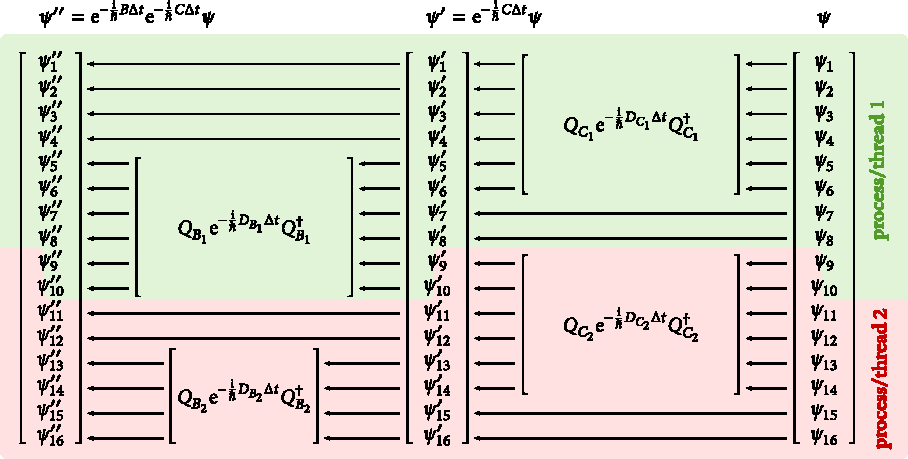
\includegraphics[width=\textwidth]{figures/numerics/parallel_split_step.pdf}
    \caption{Schematic of data flow for parallel split-step method. Computation proceeds right to left. To compute the action of $\ee^{-\frac\ii\hbar B\upDelta t}\ee^{-\frac\ii\hbar C\upDelta t}$ on a vector $\vec\psi$, one can treat the submatrices $B_1$, $B_2$, $C_1$ and $C_2$, of the block-diagonal matrices $B$ and $C$ separately. First, the exponentiation of $C$ can be applied to $\psi$ by applying the exponentiations of $C_1$ and $C_2$ to $\psi$. If diagonalisations $C_1 = Q_{C_1} D_{C_1} Q^\dagger_{C_1}$ and $C_2 = Q_{C_2} D_{C_2} Q^\dagger_{C_2}$ are known, then the two operations can be applied as a series of matrix-vector multiplications and the exponentiation of diagonal matrices. Because the two submatrices are non-overlapping, they can be applied to the vector completely independently in separate computer processes, \textsc{cpu} or \textsc{gpu} threads, or cluster nodes. The exponentiation of $B$ can then be applied to the resulting intermediate vector $\vec\psi^\prime$, similarly via two independent operations acting on nonoverlapping elements of $\psi^\prime$. However, because each submatrix of $C$ overlaps each submatrix of $B$ by $b=2$ elements on either side ($b$ being the bandwidth of the original matrix $A=B+C$), threads/processes must share these elements (here the ninth and tenth elements), sending them to each other whenever they have been updated. For simplicity this example has two compute threads and two submatrices in each term $B$ and $C$, but in general there can be any number of either. When a single thread must apply the exponentiation of multiple submatrices to the state vector, it is advantageous for it to first compute the result of any submatrix whose output is required by another thread, then all submatrices that are independent of other threads, and finally any submatrix which requires input from another thread. In this way, data required by other threads can be sent as early as possible, and data needed from other threads called upon as late as possible, minimising the time that threads are waiting for each other whilst there is useful work to be done.}
    \label{fig:parallel_split_step}
\end{figure}

Whilst this specific banded matrix $A$ is small for the sake of example, in general of course one might have a matrix of any size, allowing for $B$ and $C$ to contain more than two submatrices each. The submatrices have a minimum size of twice the bandwidth $b$ of $A$, in order to cover all elements of $A$ whilst only sharing elements with their nearest neighbour submatrices (any smaller and they would share elements with their next nearest neighbour submatrices as well, complicating things somewhat). But the only maximum is the size of $A$ itself. So what is the optimal submatrix size? Although the split-step method is still accurate to the same order in $\upDelta t$ no matter how many pieces we split a banded matrix into, we clearly introduce additional `commutation error' every time we split $A$ into additional submatrices. So one might think that the number of pieces ought be be minimised, and hence the submatrix size maximised. With regard to this, one might decide to split $A$ into $2n_\up{threads}$ submatrices (where $n_\up{threads}$ is the number of independent computational threads available), half of which will reside in $B$ and half in $C$. This minimises the extra commutation error subject to the constraint that all threads are put to use---splitting $A$ into yet smaller pieces within one computational thread will only yield unnecessary additional error.

Is this the best option? No. Despite the extra commutation error, there is additional benefit to splitting $A$ into more submatrices than required for parallelisation. Let $s$ be the `nominal' size of each submatrix, that is, the size of the corresponding \emph{non-overlapping} submatrices prior to expanding each one along the diagonal (creating overlap) by a number of elements equal to the bandwidth $b$. The computational cost of the matrix-vector multiplications for computing the action of $\ee^{-\frac\ii\hbar B\upDelta t}\ee^{-\frac\ii\hbar C\upDelta t}$ on a vector is then $\Ord{(s+b)^2}$ per submatrix, since $s+b$ is the size of the submatrices in terms of their nominal size and the bandwidth. The total number of submatrices required to cover $A$ is $ns^{-1}$, where $n$ is the size of $A$, and so the total cost of applying the exponentiations of all submatrices to a vector is $\Ord{ns^{-1}(s+b)^2}$. The cost \emph{per unit time} of simulation is then $\Ord{n\upDelta t^{-1}s^{-1}(s+b)^2}$. Here we see that splitting into smaller submatrices is desirable from the point of view of speed: because matrix-vector multiplication runs in quadratic time, a larger number of smaller matrices can be multiplied by vectors faster than a smaller number of larger matrices.

But the more submatrices, the more commutation error. Extra error can be made up for by making the timestep smaller, which increases the cost per unit time once more. So is it worth it? The extra commutation error from splitting up $A$ into more and more pieces in general depends on the form of $A$. I performed a small numerical experiment to see how the commutator $[B, C]$ (which the commutation error is proportional to) scales with $s$ for random banded matrices, as well as those corresponding to 2nd, 4th and 6th order finite differences for first and second derivatives. The result in all cases was that the commutator scaled as $s^{-\frac12}$ (see \figref{fig:commutation_error}).

\begin{figure}[t]
    \centerfloat
    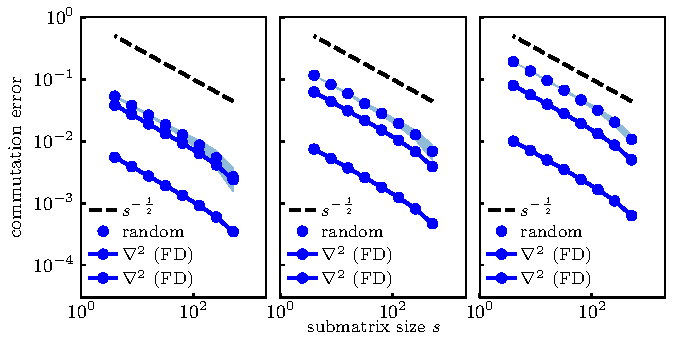
\includegraphics[width=\textwidth]{figures/numerics/commutation_error.pdf}
    \caption{Numerical experiment to determine how the commutation error scales with the submatrix size when splitting certain banded matrices into the sum of block-diagonal matrices and using a split-operator method to exponentiate the sum. From left to right, matrices with bandwidth $b=1$, $b=1$ and $b=2$ are considered. For each bandwidth, the matrices for the finite difference schemes of the order resulting in that bandwidth for first and second derivatives are considered, as well as random matrices of the given bandwidth. The random matrices have real and imaginary parts of each element within the band drawn from standard normal distributions. All matrices are $1024\times1024$. Calculations with random matrices were performed on 20 independent random matrices, and the mean and standard deviation (shaded) of the results plotted. The error metric is the \textsc{rms} element of the commutator $[B, C]$, where the orginal matrix $A$ is split into the sum of block-diagonal matrices $B + C$ using a submatrix size of $s$ (desribed in-text). The \textsc{rms} error in a vector propagated with the split-operator method is proportional this error metric. The result in all cases is that the commutator error, and therefore the error in the split-operator method scales with the submatrix size as $s^{-\frac12}$.}
    \label{fig:commutation_error}
\end{figure}

Back to our question---does decreasing the timestep size $\upDelta t$ to compensate for the additional commutation error result in more, or less computational cost per unit time than if we hadn't split $A$ into more pieces than required for parallelisation? Taking into account the nominal submatrix size $s$ and the method's error in terms of $\upDelta t$, the total error of integrating using the split-step method (assuming the $s^{-\frac12}$ commutator scaling holds) is $\Ord{\upDelta t^a s^{-\frac12}}$, where $a$ is the order in $\upDelta t$ of the accuracy of the specific split-step method used ($1$, $2$, or $4$ for those I've discussed). Using these two pieces of information: the total error, and the total cost per unit time; we can now answer the question ``What value of $s$ minimises the computational cost per unit time, assuming constant error?".

For constant error we set $\upDelta t^a s^{-\frac12} \propto 1$ and get that the computational cost per unit time at constant error is $\Ord{ns^{-\frac1{2a} - 1}(s + b)^2}$. For $a > \frac12$, this expression has a minimum at $s=b$, which is the smallest possible submatrix size in any case. For our example banded matrix $A$, decomposition into the smallest possible submatrices looks like this:
\setlength{\arraycolsep}{1pt}
\begin{align}
& A  = \left[\begin{smallmatrix}
     c & d & e &\mb&\mb&\mb&\mb&\mb&\mb&\mb&\mb&\mb&\mb&\mb&\mb&\mb\\
     b & c & d & e &\mb&\mb&\mb&\mb&\mb&\mb&\mb&\mb&\mb&\mb&\mb&\mb\\
     a & b & c & d & e &\mb&\mb&\mb&\mb&\mb&\mb&\mb&\mb&\mb&\mb&\mb\\
    \mb& a & b & c & d & e &\mb&\mb&\mb&\mb&\mb&\mb&\mb&\mb&\mb&\mb\\
    \mb&\mb& a & b & c & d & e &\mb&\mb&\mb&\mb&\mb&\mb&\mb&\mb&\mb\\
    \mb&\mb&\mb& a & b & c & d & e &\mb&\mb&\mb&\mb&\mb&\mb&\mb&\mb\\
    \mb&\mb&\mb&\mb& a & b & c & d & e &\mb&\mb&\mb&\mb&\mb&\mb&\mb\\
    \mb&\mb&\mb&\mb&\mb& a & b & c & d & e &\mb&\mb&\mb&\mb&\mb&\mb\\
    \mb&\mb&\mb&\mb&\mb&\mb& a & b & c & d & e &\mb&\mb&\mb&\mb&\mb\\
    \mb&\mb&\mb&\mb&\mb&\mb&\mb& a & b & c & d & e &\mb&\mb&\mb&\mb\\
    \mb&\mb&\mb&\mb&\mb&\mb&\mb&\mb& a & b & c & d & e &\mb&\mb&\mb\\
    \mb&\mb&\mb&\mb&\mb&\mb&\mb&\mb&\mb& a & b & c & d & e &\mb&\mb\\
    \mb&\mb&\mb&\mb&\mb&\mb&\mb&\mb&\mb&\mb& a & b & c & d & e &\mb\\
    \mb&\mb&\mb&\mb&\mb&\mb&\mb&\mb&\mb&\mb&\mb& a & b & c & d & e \\
    \mb&\mb&\mb&\mb&\mb&\mb&\mb&\mb&\mb&\mb&\mb&\mb& a & b & c & d \\
    \mb&\mb&\mb&\mb&\mb&\mb&\mb&\mb&\mb&\mb&\mb&\mb&\mb& a & b & c \\
\end{smallmatrix} \right]\nonumber\\
& =\left[ \begin{xsmallmatrix}
     c & d & e &\mb&\mb&\mb&\mb&\mb&\mb&\mb&\mb&\mb&\mb&\mb&\mb&\mb\\
     b & c & d & e &\mb&\mb&\mb&\mb&\mb&\mb&\mb&\mb&\mb&\mb&\mb&\mb\\
     a & b &c/2&d/2&\md&\mb&\mb&\mb&\mb&\mb&\mb&\mb&\mb&\mb&\mb&\mb\\
    \mb& a &b/2&c/2&\md&\md&\mb&\mb&\mb&\mb&\mb&\mb&\mb&\mb&\mb&\mb\\
    \mb&\mb&\md&\md&c/2&d/2& e &\mb&\mb&\mb&\mb&\mb&\mb&\mb&\mb&\mb\\
    \mb&\mb&\mb&\md&b/2&c/2& d & e &\mb&\mb&\mb&\mb&\mb&\mb&\mb&\mb\\
    \mb&\mb&\mb&\mb& a & b &c/2&d/2&\md&\mb&\mb&\mb&\mb&\mb&\mb&\mb\\
    \mb&\mb&\mb&\mb&\mb& a &b/2&c/2&\md&\md&\mb&\mb&\mb&\mb&\mb&\mb\\
    \mb&\mb&\mb&\mb&\mb&\mb&\md&\md&c/2&d/2& e &\mb&\mb&\mb&\mb&\mb\\
    \mb&\mb&\mb&\mb&\mb&\mb&\mb&\md&b/2&c/2& d & e &\mb&\mb&\mb&\mb\\
    \mb&\mb&\mb&\mb&\mb&\mb&\mb&\mb& a & b &c/2&d/2&\md&\mb&\mb&\mb\\
    \mb&\mb&\mb&\mb&\mb&\mb&\mb&\mb&\mb& a &b/2&c/2&\md&\md&\mb&\mb\\
    \mb&\mb&\mb&\mb&\mb&\mb&\mb&\mb&\mb&\mb&\md&\md&c/2&d/2& e &\mb\\
    \mb&\mb&\mb&\mb&\mb&\mb&\mb&\mb&\mb&\mb&\mb&\md&b/2&c/2& d & e \\
    \mb&\mb&\mb&\mb&\mb&\mb&\mb&\mb&\mb&\mb&\mb&\mb& a & b & c & d \\
    \mb&\mb&\mb&\mb&\mb&\mb&\mb&\mb&\mb&\mb&\mb&\mb&\mb& a & b & c \\
\end{xsmallmatrix} \right]
+\left[ \begin{xsmallmatrix}
    \md&\md&\md&\mb&\mb&\mb&\mb&\mb&\mb&\mb&\mb&\mb&\mb&\mb&\mb&\mb\\
    \md&\md&\md&\md&\mb&\mb&\mb&\mb&\mb&\mb&\mb&\mb&\mb&\mb&\mb&\mb\\
    \md&\md&c/2&d/2& e &\mb&\mb&\mb&\mb&\mb&\mb&\mb&\mb&\mb&\mb&\mb\\
    \mb&\md&b/2&c/2& d & e &\mb&\mb&\mb&\mb&\mb&\mb&\mb&\mb&\mb&\mb\\
    \mb&\mb& a & b &c/2&d/2&\md&\mb&\mb&\mb&\mb&\mb&\mb&\mb&\mb&\mb\\
    \mb&\mb&\mb& a &b/2&c/2&\md&\md&\mb&\mb&\mb&\mb&\mb&\mb&\mb&\mb\\
    \mb&\mb&\mb&\mb&\md&\md&c/2&d/2& e &\mb&\mb&\mb&\mb&\mb&\mb&\mb\\
    \mb&\mb&\mb&\mb&\mb&\md&b/2&c/2& d & e &\mb&\mb&\mb&\mb&\mb&\mb\\
    \mb&\mb&\mb&\mb&\mb&\mb& a & b &c/2&d/2&\md&\mb&\mb&\mb&\mb&\mb\\
    \mb&\mb&\mb&\mb&\mb&\mb&\mb& a &b/2&c/2&\md&\md&\mb&\mb&\mb&\mb\\
    \mb&\mb&\mb&\mb&\mb&\mb&\mb&\mb&\md&\md&c/2&d/2& e &\mb&\mb&\mb\\
    \mb&\mb&\mb&\mb&\mb&\mb&\mb&\mb&\mb&\md&b/2&c/2& d & e &\mb&\mb\\
    \mb&\mb&\mb&\mb&\mb&\mb&\mb&\mb&\mb&\mb& a & b &c/2&d/2&\md&\mb\\
    \mb&\mb&\mb&\mb&\mb&\mb&\mb&\mb&\mb&\mb&\mb& a &b/2&c/2&\md&\md\\
    \mb&\mb&\mb&\mb&\mb&\mb&\mb&\mb&\mb&\mb&\mb&\mb&\md&\md&\md&\md\\
    \mb&\mb&\mb&\mb&\mb&\mb&\mb&\mb&\mb&\mb&\mb&\mb&\mb&\md&\md&\md\\
\end{xsmallmatrix} \right].
\end{align}

So the conlusion is: use the smallest submatrices possible when decomposing a banded matrix into a sum of two block-diagonal matrices. The decrease in computational costs, even when the increased error is compensated for by a smaller timestep, is worth it.

\subsubsection{Limitations and nonlinearity}\label{sec:limitations_nonlinearity}

The split-step method is quite powerful and general. It allows you to approximately decompose the exponentiation of a Hamiltonian into exponentiations of its component terms, in the subspaces that they act on, and avoids exponentiating large banded matrices; saving on computing power immensely compared to exponentiating the full Hamiltonian. It is unitary (when the Hamiltonian is actually Hermitian), and stable---that is, unlike Runge--Kutta methods, the method's truncation error does not grow without limit but is bounded (disregarding floating point rounding error, which is much smaller than the truncation error of either method) \cite{schneider_parallel_2006}. So there is no need to take much smaller timesteps than one otherwise would at earlier times in order to ensure the error remains acceptable at later times---an appropriate timestep at earlier times will be appropriate at later times, \emph{ceteris paribus}. This is extremely appealing. And, whilst higher order split-step methods quickly become unwieldy \cite{schneider_parallel_2006}, fourth order accuracy is quite acceptable for many problems.

Applying all the tricks described in the above sections results in $\Ord{\upDelta t}$, $\Ord{\upDelta t^2}$ and $\Ord{\upDelta t^4}$ accurate timestepping methods for solving the Schr\"odinger equation with total computational cost scaling as $\Ord{n \sum_i b_i}$, where $n=\prod_i n_i$ (for a product space of subspaces with dimensionalities $\{n_i\}$) is the dimensionality of the total Hilbert space, and $\{b_i\}$ are the bandwidths of the matrix representations of each term in the Hamiltonian in the chosen basis.\footnote{Now that we are here, we can finally say something about the best basis for simulating in: to minimise computational costs, the best basis is the one that minimises precisely this sum of bandwidths. The exception to this is when fast Fourier transforms are involved, which I discuss later.} Furthermore, the method is efficiently parallelisable, provided the the maximum size-to-bandwidth ratio $\max_i(n_i/b_i)$ of the terms in the Hamiltonian is much larger than the number of parallel computing threads available. Although the constant factors that big-O notation neglects may not be optimal, this scaling would seem to be the best one could hope for---for each of the $n$ elements in the state vector one must consider the $\sum_i b_i$ elements (including itself) that the Hamiltonian couples it with, and no more.\footnote{Assuming the banded matrices are otherwise dense within their band---further improvements would be possible if some elements within the band were always zero.}

The main downside of this otherwise excellent method of exponentiating Hamiltonians is that the evolution modelled must actually be described by a linear system of equations. One cannot add arbitrary terms and nonlinear operators to the Hamiltonian, as the split-step method requires that one can evaluate each time-dependent term in the Hamiltonian at specific times, including times at which the solution for the state vector is not yet available. This would seem to limit the split-step method strictly to modelling \emph{linear} dynamics, that is, terms in the Hamiltonian must not depend explicitly on the state vector they are operating on. Whilst nature might fundamentally be described by linear dynamics, once approximations of various kinds are made in order to make problems tractable, it's extremely common to end up with a nonlinear pseudopotential or nonlinear effective Hamiltonian. Note that non-\emph{Hermitian}, pseudo-Hamiltonians---leading to non-unitary evolution---are fine. The split-step method has made no assumptions that rules them out, it only assumes the differential equation can be expressed in the form
\begin{align}
\dv t \vec\psi(t) = \sum_n H_n(t)\vec\psi(t),
\end{align}
where $\{H_n\}$ are a set of linear operators, Hermitian or not.

Fortunately, one specific form of nonlinearity that cold atom physicists are particularly interested in---the nonlinear term in the Gross--Pitaevskii equation---can be incorporated without much difficulty. As mentioned, the problem with nonlinearity is that all but the first-order split step methods require you to evaluate terms in the Hamiltonian at some future time at which the state vector is not yet known, that is the algorithm contains steps akin to $\vec \psi(t_{n+1}) = U(t_{n+1}, t_n; \vec\psi(t_{n+1})) \vec \psi(t_n)$ for some nonlinear unitary matrix $U(t_{n+1}, t_n; \vec\psi(t_{n+1}))$---$U$ cannot be explicitly constructed because it both requires and is required by $\psi(t_{n+1})$.

For the Gross--Pitaevskii effective Hamiltonian, the second-order split-step method (from which the fourth order method is constructed) for a single step might be na\"ively written
\begin{align}
\vec \psi(t_{n+1}) =
\ee^{-\frac\ii\hbar K \frac{\upDelta t} 2}
\ee^{-\frac\ii\hbar (g\rho(t_{n+1}) + V(t_{n+1})) \frac{\upDelta t} 2}
\ee^{-\frac\ii\hbar (g\rho(t_n) + V(t_n) ) \frac{\upDelta t} 2}
\ee^{-\frac\ii\hbar K \frac{\upDelta t} 2}
\vec \psi(t_n),
\end{align}
where $\vec\psi(t)$ is the state vector\footnote{Usually when modelling the GPE the single-particle state vector is normalised to the number of particles, rather than unity, and so strictly speaking it cannot be called a state vector, though it otherwise can be treated as one in most respects.} represented in a discrete position basis, $g$ is the nonlinear interaction constant, $V(t)$ and $\rho(t) = \vec\psi(t)\vec\psi^\dagger(t)$ are diagonal matrices for the external potential and the density matrix for $\vec\psi(t)$ in the same position basis, and $K$ is a discrete approximation to the kinetic energy operator in the position basis.

As written, this can't be evaluated because $\vec \psi(t_{n+1})$---required to evaluate $\rho(t_{n+1})$---is not yet known. The order we choose to exponentiate the terms in our Hamiltonian is arbitrary, however (so long as we alternately reverse that order each half-step as required by the second order split-step method),
and so swapping the order gives
\begin{align}
\vec \psi(t_{n+1}) =
\ee^{-\frac\ii\hbar (g\rho(t_{n+1}) + V(t_{n+1})) \frac{\upDelta t} 2}
\ee^{-\frac\ii\hbar K \upDelta t}
\ee^{-\frac\ii\hbar (g\rho(t_n) + V(t_n) ) \frac{\upDelta t} 2}
\vec \psi(t_n),
\end{align}
which incidentally has the benefit that since $K$ is (ordinarily) time independent, the two adjacent exponentials containing it can be combined into one. Now $\rho(t_{n+1})$ is contained within the leftmost exponential, and so it is the last operator to be applied in the timestep. Note that since $g\rho(t)$ is real and diagonal in the position basis (as is $V(t)$), ths leftmost unitary merely changes the phase of the state vector at each point in space, having no effect on its density. This means that $\rho(t)$ is, in fact, unaffected by this last unitary evolution operator. Hence, $\rho(t_{n+1})$ can be computed simply as the density matrix of the intermediate state vector that this unitary was to act on:
\begin{align}
\rho(t_{n+1}) = \vec\psi(t_{n+1})\vec\psi^\dagger(t_{n+1}) = \tilde{\vec\psi}\tilde{\vec\psi}^\dagger,
\end{align}
where
\begin{align}
\tilde{\vec\psi} = 
\ee^{-\frac\ii\hbar K \upDelta t}
\ee^{-\frac\ii\hbar (g\rho(t_n) + V(t_n) ) \frac{\upDelta t} 2}
\vec \psi(t_n).
\end{align}

The inclusion of $V(t)$ with $g\rho(t)$ is optional, and if $V(t)$ was not real valued, would not be valid (since in that case the density \emph{would} be affected by the evolution induced by $V(t)$). In such a case the Hamiltonian would have to be split into three terms with $V(t)$ and $g\rho(t)$ treated separately.

So now we can put some conditions on what types of nonlinear operators can be used within the second-order split step method. The first condition is that at most one nonlinear operator can be included, since it must be placed last in the sandwich of exponentials (otherwise its value at the end of the timsestep cannot be inferred immediately prior to acting on the state vector). The second condition is that the nonlinear operator must be invariant with respect to the evolution that it itself induces in the state vector. Here we have an operator that  depends only on the state vector's absolute value, but for which the corresponding unitary only evolves the state vector's phase. Another example might be an operator that depends only on the state vector's phase gradients, but evolves the state vector's absolute value, and so forth.

Although I find this argument compelling for second-order split-step, it's less obvious that it should hold for fourth-order split-step as well, which, even though it is based on multiple applications of second-order split-step, involves a substep that is backwards in time. `Evaluate the nonlinear operator based on the state vector at this specific time' becomes ambiguous when that moment in time is traversed in both directions by two different sub-steps. However, \cite{javanainen_symbolic_2006} have verified using computer symbolic algebra that indeed, up to even higher order split-step methods, putting the nonlinear density term last in the splitting and always evaluating it using the value of the intermediate state vector immediately prior results in the method having the same order accuracy in $\upDelta t$ as for linear operators only. Given this and my argument above, as well as the reasoning that the second-order split-step method has no way of `knowing' whether it is acting backward in time or not when embedded in a higher-order split step method, I would expect the same to hold for all nonlinear operators meeting the above two conditions, though I haven't shown this explicitly.

\section{For everything else, there's fourth-order Runge--Kutta}\label{sec:rk4}

Fourth-order Runge--Kutta (\textsc{rk4}) is the enduring workhorse of numerical integration methods. Of the Runge--Kutta methods, it offers a good balance of accuracy and computational cost. When a problem does not have the properties that allow manifestly unitary or error-bounded methods to be used, or when enough computing power can be deployed so as to make these concerns irrelevant, and the programmer's time more important, fourth order Runge--Kutta is a good choice.

It is not manifestly unitary, and its error is not bounded. For a given integration step size, the error will eventually diverge exponentially. This divergence can be delayed, but not prevented, by decreasing the step size. Nonetheless for many problems this is not a concern in practice.

The advantages of fourth-order Runge--Kutta are compelling: it's global error is fourth order in the integration timestep, involves four function evaluations per timestep, requires only linear arithmetic operations outside of the function evaluations, and can be applied any problem that can be written in the form
\begin{align}
\dv t \vec x = f(\vec x, t),
\end{align}
for some (possibly nonlinear) function $f$, where $\vec{x}$ is a vector of dynamical variables, often in our case the components of a state vector, or for classical dynamics the positions and velocities of an ensemble of particles\footnote{For classical particle dynamics, often lower order symplectic methods such as the leapfrog method [CITE] can be preferable, but nonetheless it is hard to overstate the usefulness of a general purpose algorithm such as \textsc{rk4} that can be deployed as a first attempt, or as a plan B once the assumptions required by another algorithm are violated}. Note that this formation allows for initial value problems with coupled \textsc{ode}s, discretised \textsc{pde}s, as well as second or higher order differential equations, since an equation of the form
\begin{align}
\dv[2] t \vec x = f(\vec x, t)
\end{align}
can be rewritten
\begin{align}
\dv t \left(\vec x, \dot{\vec x}\right) = \left(\dot{\vec x}, f(\vec x, \dot{\vec x}, t)\right),
\end{align}
treating the time derivative of each element of $\vec x$ as simply another coupled dynamical variable.

Not unrelated to its ease of implementation, the method itself can be stated concisely. Propagation of the dynamical variables for one timestep from time $t$ to time $t + \upDelta t$ is computed as follows:
\begin{align}
\vec k_1 &= f(\vec x(t), t),\nonumber\\
\vec k_2 &= f(\vec x(t) + \tfrac12 \vec k_1\upDelta t, t + \tfrac12\upDelta t),\nonumber\\
\vec k_3 &= f(\vec x(t) + \tfrac12 \vec k_2\upDelta t, t + \tfrac12\upDelta t),\nonumber\\
\vec k_4 &= f(\vec x(t) + \vec k_3\upDelta t, t + \upDelta t),\nonumber\\
\vec x(t + \upDelta t) &= \vec x(t)
+ \tfrac{\upDelta t}6(\vec k_1 + 2\vec k_2 + 2\vec k_3 + \vec k_4).\label{eq:rk4}
\end{align}

Each step is self-contained, that is, the algorithm does not contain any state from previous steps. This is appealing as it means that $f$ can change discontinuously between timesteps without giving rise to Runge's phenomenon [CITE] in the approximate solutions $\vec x(t)$, as can be the case with multistep methods which do retain some dependency on previous steps.
$\vec x(t)$ can also be modified discontinuously between steps without causing problems, as is required by Monte-Carlo wavefunction or quantum jump methods [CITE], or even in the imaginary time evolution method [SEE SECTION SECREF] which requires normalisation of the state vector in between steps. Fourth order Runge--Kutta is therefore quite compatible with stochastic processes and many other models which may not be described by a differential equation alone.

One downside is that the timestep used must be much smaller than the timescale on which $\vec x$ changes - even if $\vec x$'s time variation is highly regular. If $x$'s time variation is dominated by the simple accumulation of complex phase at some angular frequency---as is often the case in quantum mechanics---the timesteps used for \textsc{rk4} must be small enough to resolve these circles about the complex plane. This is in contrast to the exponentiation methods, for which an energy offset (and hence overall change in the angular frequency at which the state vector's elements accumulate phase) is largely irrelevant. Energy offsets or use of an interaction picture can mitigate this problem but requires some foresight, and may not be possible if the required energy offsets change in time or are not known analytically in advance. The method I develop in section [SECREF] is a partial remedy for this specific problem, which in my opinion is the biggest weakness of fourth order Runge--Kutta as applied to quantum state evolution, when compared to the unitary methods.

\subsection{Complexity and parallelisability for the Schr\"odinger equation}

Excluding the evaluation of $\vec f$, \textsc{rk4} requires a number of arithmetic operations proportional to the number of elements in $\vec x$, and so contributes time-complexity $\Ord{n}$ to the overall calculation, where $n$ is the number of elements in $\vec x$. Since $f$ itself usually doesn't run in linear time, the computational time complexity of \textsc{rk4} is usually therefore that of evaluating $f$. Its parallelisability also comes down to that of $f$, since equations (\ref{eq:rk4}) above treat each element of $\vec x$ completely independently, with any couplings computed within $f$.

For the Schr\"odinger equation in a concrete basis, $f$ is
\begin{align}
f(\vec \psi, t) = -\frac\ii\hbar H(t)\vec \psi,
\end{align}
where $\vec \psi$ is the state vector in the given basis and $H(t)$ is the matrix representation of the Hamiltonian in that basis\footnote{For the Gross--Pitaevskii equation this would be a nonlinear $H(\vec \psi, t)$, and everything else in this section still applies.}. Fourth order Runge--Kutta is therefore as computationally expensive and parallelisable as computing the matrix-vector product $H(t)\vec\psi$. In the worst case this multiplication is $\Ord{n^2}$ in the size of the Hilbert space and barely parallelisable at all, if $H$ is dense. But in the common case (as mentioned in section \ref{sec:split-step}), of $H$ being a sum of terms which act on different subspaces, i.e.
\begin{align}
H(t) = \sum_{i=1}^N \mathbb{I}_{n_1} \otimes \cdots  \otimes \mathbb{I}_{n_{i-1}}
\otimes  H_i(t) \otimes  
 \mathbb{I}_{n_{i+1}} \otimes \cdots \otimes \mathbb{I}_{n_N}
\end{align}
where $n_i$ is the dimensionality of the subspace acted on by the $i^\up{th}$ term and $\mathbb{I}_m$ is the $m\times m$ identity matrix, then things are much better. If each term is dense, then the overall cost of evaluating the product $H(t)\vec\psi$ is $\Ord{n\sum_i n_i}$, where $n = \prod_i n_i$ is the dimensionality of the total Hilbert space, which can be considerably less than the $\Ord{n^2}$ of evaluating the single  matrix-vector product for the total Hamiltonian. And if each term is a banded matrix with bandwidth $b_i$, then the cost of applying a single term in the Hamiltonian becomes $\Ord{n b_i}$ instead of $\Ord{n n_i}$, and so the cost of evaluating $H(t)\vec\psi$ becomes $\Ord{n\sum_i b_i}$. This is identical to the earlier result for the split-operator method once the trick of splitting up banded matrices into block-diagonal matrices was applied (section [SECREF]), but with much less work. Representing $H(t)$ as a sum of terms over different subspaces is no extra work---this is the form we are likely to be writing Hamiltonians in already, and constructing the total $H(t)$ is often not useful. Have you ever considered constructing the matrix form of say, $\frac {\hat p_x^2} {2m} + \frac {\hat p_y^2} {2m}$ for some finite difference or pseudospectral representations of $\hat p_x$ and $\hat p_y$? I can't think of a reason to do so. No, we are already applying these operators to different subspaces of the Hilbert space and then summing the results without thinking twice about it, and so the above analysis mostly serves as a reminder that what we are already doing most of the time is in fact very efficient. 

Parallelisation, provided one or more of the matrices are banded, is also straightforward, since if $A$ is banded with bandwidth $b$, then
\begin{align}
(A \vec \psi)_i = \sum_{j=-b}^b A_{i, i+j} \psi_j,
\end{align}
that is, calculation of an element of $A\vec\psi$ requires only the corresponding element of $\vec \psi$ and its nearest $b$ neighbours on each side. One can therefore divide up the state vector into contiguous regions (in the subspace in which $A$ acts), and compute different elements of the product on different compute threads, requiring an exchange of only $b$ elements at each boundary\footnote{A note about minimising the effect of latency: at the start of an \textsc{rk4} substep, have each thread send the required elements at the edges of its region in each subspace to its neighbouring threads \emph{first}. \emph{Then} compute $H(t)\vec\psi$ on the interior elements. If each thread has a sufficiently large workload, then by the time this is complete, the data from neighbouring regions will have arrived and threads will not have spent any time waiting for each other.} between neighbouring threads.

An additional benefit of parallelised \textsc{rk4} when compared to split-operator is that the same amount of data needs to be sent between threads regardless of the number of terms in the Hamiltonian. In split-step methods, each term in the Hamiltonian is exponentiated separately (multiple times for the higher order schemes), requiring an exchange of data each time. The amount of data needing to be exchanged per step therefore scales with the number of terms in the Hamiltonian being parallelised, whereas for \textsc{rk4} it is constant.

The constant factors that big-O notation disregards also favour \textsc{rk4} when compared to split-operator methods. For one, addition and multiplication are much cheaper than exponentiation, meaning that the exponentials in split-operator methods may add considerable computational cost if the Hamiltonian itself is simple. Furthermore, parallelised or not, each term in fourth order split-operator adds $20$ matrix-vector products in the space the term acts, whereas \textsc{rk4} requires only one additional matrix-vector product per term. In practice due to these properties, \textsc{rk4} runs considerably faster than split-operator methods, even for simple systems, and the gap widens as complexity increases.

% \subsection{The interaction picture}

% A common situation in atomic physics is to be simulating the internal state of an atom, armed with the knowledge that only a small number of atomic states are able to become occupied.

%         \begin{itemize}
%             \item Sometimes called a "rotating frame"
%             \item Is equivalent to basis change where new basis functions differ by a time-dependent phase factor
%             \item Is defined by a time-independent Hamiltonian
%             \item This has the effect of moving some time dependence into the operators (demonstrate, by writing some operators with the unitary in front of them. As you can see it is simply a change of basis - but a time-dependent one.)
%             \item No need to remain in the same interaction picture - can be redefined arbitrarily often throughout a simulation and state vectors transformed into new basis.
%         \end{itemize}
% \begin{itemize}

% \item {absorbing boundary conditions, reflective boundary conditions, periodic boundary conditions}

% \end{itemize}

\section{Continuous degrees of freedom}\label{sec:continuous_dof}
The single-particle, non-relativistic, scalar Schr\"odinger wave equation, as distinct from the general Schr\"odinger equation \eqref{eq:schrodinger_equation}, is:
\begin{align}\label{eq:schrodinger_wave_equation}
\ii\hbar\pdv{}{t}\psi(\vec r, t) = \left[-\frac{\hbar^2}{2m} \nabla^2 + V(\vec r)\right]\psi(\vec r, t).
\end{align}
Sinilarly, ss mentioned in [SECREF INTRODUCTION], the equation for the single-particle wavefunction of an atom in a single-component Bose--Einstein condensate is the Gross--Pitaevskii equation
\begin{align}
\ii\hbar\pdv{}{t}\psi(\vec r, t) = \left[-\frac{\hbar^2}{2m} \nabla^2 + V(\vec r) + g\abs{\psi(\vec r, t)}^2\right]\psi(\vec r, t),
\end{align}
where $\psi(\vec r, t) = \sqrt{N}\braket{\vec r}{\psi(t)}$ is the single-particle wavefunction scaled by the square root number of atoms $N$.

Both these equations are partial differential equations involving both spatial and temporal derivatives. But in numerical quantum mechanics all state vectors are mapped to column vectors and all operators to matrices. Spatial wavefunctions are no exception to the former and differential operators such as $\grad^2$ are no exception to the latter--these objects can be thought of as infinite-dimensional vectors and matrices. So the above two equations are the general Schr\"odinger equation \eqref{eq:schrodinger_equation}, given specific Hamiltonians, an represented in a concrete---albeit infinite-dimensional--basis. But we can only perform a finite number of computations, so what do these vectors and operators look like once we reduce them to something finite? That depends on whether we choose to discretise space on a grid, or use a functional basis (and on which functional basis we choose). As we'll see, however, spatial discretisation is actually just a special case of a functional basis, namely the Fourier basis, plus an additional approximation or two. The resulting matrices are \emph{banded}, justifying the previous two sections' obsession with dealing with banded matrices efficiently.

\subsection{Spatial discretisation on a uniform grid: the Fourier basis}

Imagine a two dimensional spatial region within which we are solving the single-component Gross--Pitaevskii equation, evolving an initial condensate wavefunction in time. Having specified which degrees of freedom we want to simulate (two continuous degrees of freedom, one for each spatial dimension), the next step according to the method outlined in section \ref{sec:neglect_discretisation} is to choose a basis in which to represent this state vector.

Let's say we discretise space in an equally-spaced $n_x\times n_y = 7\times 7$ rectangular grid,\footnote{For the sake of example---$256\times256$ is a more realistic minimum.} with spacings $\upDelta x$ and $\upDelta y$, and only represent the wavefunction at those $49$ points in space. The state vector can then be represented by a list of $49$ complex numbers, each taken to be the wavefunction's value at the spatial position corresponding to one gridpoint. This $49$-vector is now a concrete representation of our state vector (\figref{fig:vector_unravel}).

\begin{figure}[t]
    \centerfloat
    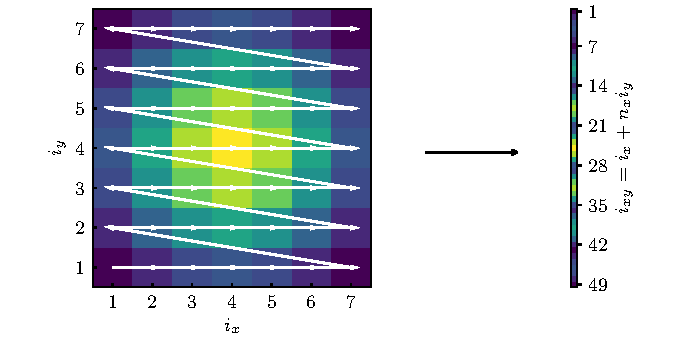
\includegraphics[width=\textwidth]{figures/numerics/vector_unravel.pdf}
    \caption{Discretising a function over two dimensional space on a grid yields a list of coefficients, one for each gridpoint. These can be arranged as a column vector, and in this way a two dimensional wavefunction approximated by a finite-dimensional state vector. Computationally we don't normally treat this state vector as a column vector---it is more convenient to leave it as a two-dimensional array. But conceptually it is a single vector living in the product space of the discretised $x$ and $y$ spaces.}
    \label{fig:vector_unravel}
\end{figure}

\begin{figure}[t]
    \centerfloat
    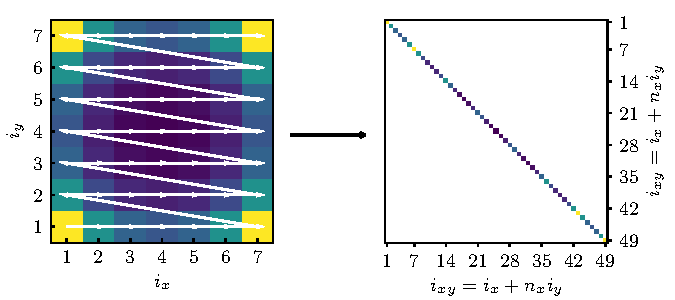
\includegraphics[width=\textwidth]{figures/numerics/potential_unravel.pdf}
    \caption{[Potential unravelling]}
    \label{fig:potential_unravel}
\end{figure}

We can also evaluate the potential (and nonlinear term in the case of the Gross--Pitaevskii equation) at each gridpoint and declare this a diagonal operator (\figref{fig:potential_unravel}). Finally, we could use finite differences to compute the Laplacian - equivalent to replacing the Laplacian with a matrix
\begin{align}
L = L_x \otimes \mathbb{I}_{n_y} + \mathbb{I}_{n_x} \otimes L_y 
\end{align} 
where $L_x$ and $L_y$ are (banded) matrices for finite difference approximations to second derivatives in each direction. We might also use discrete Fourier transforms to evaluate the Laplacian, since
\begin{align}
\nabla^2\psi(\vec r) = \mathcal{F}^{-1}\left\{-k^2\mathcal{F}\{\psi(\vec r)\}(\vec k)\right\},
\end{align}
where $ k = \abs{\vec k}$.

This is all well and good, and it works. But at what point did we choose a basis just now---what are the basis vectors? This just looks like discretising space at a certain resolution, rather than the formal process of choosing a basis and projecting the state vector and operators onto each basis vector, as outlined in section \ref{sec:neglect_discretisation}. Assuming what we've done is equivalent to choosing a basis, that basis has a finite number ($49$) of basis vectors, which means it cannot be complete, since state vectors we're approximately representing with it require an infinite number of complex numbers to be described exactly.\footnote{One for each position within the two dimensional space we're representing.} So what do the basis functions look like, and what state vectors have we implicitly excluded from simulation by choosing a basis that is incomplete?

Prior to discretising, the spatial wavefunction $\psi(\vec r, t) = \braket{\vec r}{\psi(t)}$ was already the representation of the abstract state vector $\ket{\psi}$ in the ``spatial basis"---a basis in which the basis vectors $\{\ket{\vec r}\}$ are Dirac deltas positioned at each point in space. The value of the wavefunction $\psi(\vec r)$ for a specific $\vec r$ is then simply a coefficient saying how much of the basis vector $\ket{\vec r}$ to include in the overall state vector. What we have \emph{not} done is chosen a subset of these Dirac delta basis functions as our basis. This would be very strange---our representation of the wavefunction would allow it to be nonzero at the gridpoints, but not in between, like a comb. Spatially separated Dirac deltas do not spatially overlap at all; the matrix elements of the kinetic energy operator:
\begin{align}
\matrixel{\vec r_i}{\hat K}{\vec r_j} = \int \delta(\vec r - \vec r_i)\left(-\frac{\hbar^2}{2m}\grad^2\right)\delta(\vec r - \vec r_j)\,\dd \vec r
\end{align}
would all be zero for $i\neq j$, disallowing any flow of amplitude from one point in space to another by virtue of it not being able to pass through the intervening points.

Neither have we implicitly chosen a set of two-dimensional boxcar functions centred on each gridpoint with width $\upDelta x$ and $\upDelta y$ in each direction respectively. These cover all space in between gridpoints, but are are not twice differentiable everywhere, and hence the kinetic energy operator's matrix elements cannot be evaluated\footnote{Delta functions aren't twice differentiable either, so this itself isn't a fatal flaw--but even if one defines the boxcar functions as the limit of twice differentiable functions becoming increasingly square with some parameter, the limit for the kinetic energy matrix elements between adjacent boxcars goes to infinity.}. No, neither of these bases makes sense. To interpret our spatial grid as a basis, we need a set of functions $\phi_{ij}(r)$ (where $i$ and $j$ are the indices of the gridpoints in the $x$ and $y$ directions respectively) that are orthonormal, are nonzero only at one gridpoint and are zero at all others, and are twice differentiable everywhere in our spatial region. Infinite choices are available, differing in which subspace of the original Hilbert space they cover. A sensible heuristic for choosing one is that we want to be able to represent the state vectors whose wavefunctions do not change much between adjacent gridpoints, and we are happy for the necessary incompleteness of our basis to exclude wavefunctions with any sort of structure in between gridpoints.

\subsubsection{The discrete Fourier transform to the rescue}

It turns out that discretising space in this way can indeed be equivalent to choosing a sensible basis. This is made clearer by first discretising in Fourier space instead, and seeing how this can imply a discretisation in real space.

One possible basis for representing all possible state vectors is the Fourier basis $\{\ket{\vec k_{ij}}\}$. With it, any state vector (whose wavefunction is nonzero only within the \textsc{2d} region) can be represented as the sum of basis vectors whose wavefunctions are \textsc{2d} plane waves, also localised to the 2D region:
\begin{align}\label{eq:spatial_plane_wave_basis}
\braket{\vec r}{\vec k_{ij}} = \begin{cases}
\frac 1 {\sqrt A} e^{i\vec k_{ij}\cdot\vec r}\qquad (\vec r\ \textrm{within \textsc{2d} region})\\
0\qquad(\vec r\ \textrm{not within \textsc{2d} region}),
\end{cases}
\end{align}
where $A$ is the area of the \textsc{2d} region and the wavevector of each plane wave is
\begin{align}
\vec k_{ij} = \left[ \tfrac {2\pi i}{L_x}, \tfrac {2\pi j}{L_y}\right]^\up{T},
\end{align}
where $i$ and $j$ are (possibly negative) integers. Any state vector whose wavefunction is localised to the \textsc{2d} region can then be written as the infinite sum:
\begin{align}
\ket\psi &= \sum_{i=0}^\infty\sum_{j=0}^\infty \braket{\vec k_{i,j}}\psi \ket{\vec k_{i,j}}\\
\Rightarrow \psi(\vec r) &= \braket{\vec r}{\psi} = \begin{cases}
\sum_{i=0}^\infty\sum_{j=0}^\infty \braket{\vec k_{ij}}\psi \frac 1 {\sqrt A} e^{i\vec k_{ij}\cdot\vec r}
\qquad (\vec r\ \textrm{within \textsc{2d} region})\\
0\qquad(\vec r\ \textrm{not within \textsc{2d} region}).
\end{cases}
\end{align}
So $\{\braket{\vec k_{ij}}\psi\}$ are simply the coefficients of the \textsc{2d} Fourier series of $\psi(\vec r)$.

What does this have to do with our discretised space? These basis functions $\{\braket{\vec r}{\vec k_{ij}}\}$ don't have the required properties for a spatial discrete basis. For one, there are an infinite number of them, and we require 49 for our 7$\times$7 example. Secondly, all of them are nonzero everywhere within the \textsc{2d} region, whereas we require each basis function to be nonzero at exactly one of out 25 gridpoints.

We can solve the first problem by truncating the Fourier series. By only including basis vectors $\ket{\vec k_{ij}}$ for which:
\begin{align}
\begin{cases}
i \in [-\tfrac{n_x}2, \tfrac{n_x}2 - 1] \qquad (n_x\ \textrm{even})\\
i \in [-\tfrac{n_x - 1}2, \tfrac{N_x - 1}2] \qquad (n_x\ \textrm{odd})
\end{cases}
\end{align}
and
\begin{align}
\begin{cases}
j \in [-\tfrac{n_y}2, \tfrac{n_y}2 - 1] \qquad (n_y\ \textrm{even})\\
j \in [-\tfrac{n_y - 1}2, \tfrac{n_y - 1}2] \qquad (n_y\ \textrm{odd})
\end{cases}
\end{align}
we include only the $n_x$ and $n_y$ longest wavelengths in each respective spatial dimension. This is a sensible truncation with a physically meaningful interpretation. By making it, we are no longer able to represent state vectors with short wavelength components. Because the kinetic energy operator, when represented in the Fourier basis, is:
\begin{align}
\matrixel{\vec k_{ij}}{\hat K}{\vec k_{i^\prime j^\prime}} = \frac{\hbar^2 k^2}{2m}\updelta_{ii^\prime}\updelta_{jj^\prime},
\end{align}
where $k = |\vec k_{ij}|$, by excluding basis vectors with larger wavevectors, we are excluding state vectors with large kinetic energy. Thus the truncation is a kinetic energy cutoff, and is an accurate approximation whenever a simulation is such that the system is unlikely to obtain kinetic energies above the cutoff.\footnote{Because a \emph{square} region in Fourier space is being carved out, by limiting each of $k_x$ and $k_y$ to finite ranges rather than the total wavenumber $k = \sqrt{k_x^2 + k_y^2}$, there is no single kinetic energy cutoff so to speak. Nonetheless there is a maximum wavenumber $k_\up{max} = \min(\{|k_x|\} \cup \{|k_y|\})$ defining a kinetic energy cutoff $K_\up{max} = \hbar^2k_\up{max}^2/(2m)$ below which kinetic energies definitely are representable and above which they may not be.} It also matches our earlier intuition that our basis should represent wavefunctions that don't vary much between gridpoints---here we are discarding short wavelengths and hence limiting wavefunctions we can represent to ones that vary slowly in space compared to the cutoff wavelength.

Now we have a set of basis vectors---a discrete Fourier basis---but their spatial wavefunctions still don't have the property of being nonzero only at a single gridpoint each. On the contrary, each plane wave has has a constant amplitude everywhere in space. But consider the following superposition of Fourier basis vectors:
\begin{align}\label{eq:DFT_basischange}
\ket{\vec r_{ij}} = \sum_{i^\prime}^{n_x}\sum_{j^\prime}^{n_y} e^{-i \vec k_{i^\prime j^\prime} \cdot \vec r_{i j}}\ket{\vec k_{i^\prime j^\prime}}
\end{align}

with $\vec r_{i j} = (i \upDelta x, j \upDelta y)^\up{T}$ and. The set of vectors $\{\ket{\vec r_{i, j}}\}$ are also an orthonormal basis, related to the discrete Fourier basis by a unitary transformation with matrix elements:
\begin{align}
U_{\textsc{dft2}, i^\prime j^\prime ij} = \braket{\vec k_{i^\prime j^\prime}}{\vec r_{i j}} = e^{-i \vec k_{i^\prime j^\prime} \cdot \vec r_{i j}}.
\end{align}

This unitary transformation is in fact a two-dimensional discrete Fourier transform (hence the subscript), and the basis vectors $\{\ket{\vec r_{ij}}\}$ have spatially localised wavefunctions that are nonzero only at one of the spatial gridpoints. Vectors and matrices can be transformed from their discrete Fourier space representation to their discrete real-space representation and back using the unitary $U_{\textsc{dft2}}$:

\begin{align}
\vec\psi_\up{real} &= U^\dagger_{\textsc{dft2}} \vec \psi_\up{Fourier}\\
\vec\psi_\up{Fourier} &= U_{\textsc{dft2}} \vec \psi_\up{real}\\
A_\up{real} &= U^\dagger_{\textsc{dft2}} A_\up{Fourier} U_{\textsc{dft2}}\\
A_\up{Fourier} &= U_{\textsc{dft2}} A_\up{Real} U^\dagger_{\textsc{dft2}}.
\end{align}
where $\vec\psi_\up{real}$ is the vector of coefficients $\psi_{\up{real},ij}= \braket{\vec r_{ij}}{\psi}$ for representing a state vector in the discrete real space basis, $\vec\psi_\up{Fourier}$ is the vector of coefficients $\psi_{\up{Fourier}, ij} = \braket{\vec k_{ij}}{\psi}$ for the state vector in the discrete Fourier basis, and $A_\up{real}$ and $A_\up{Fourier}$ are the representations of some operator $\hat A$ in the discrete real and Fourier bases respectively, with matrix elements $A_{\up{real}, ij i^\prime j^\prime} = \matrixel{\vec r_{ij}}{\hat A}{\vec r_{i^\prime j^\prime}}$ and $A_{\up{Fourier},ij i^\prime j^\prime} = \matrixel{\vec k_{ij}}{\hat A}{\vec k_{i^\prime j^\prime}}$.

\begin{figure}[t]
    \centerfloat
    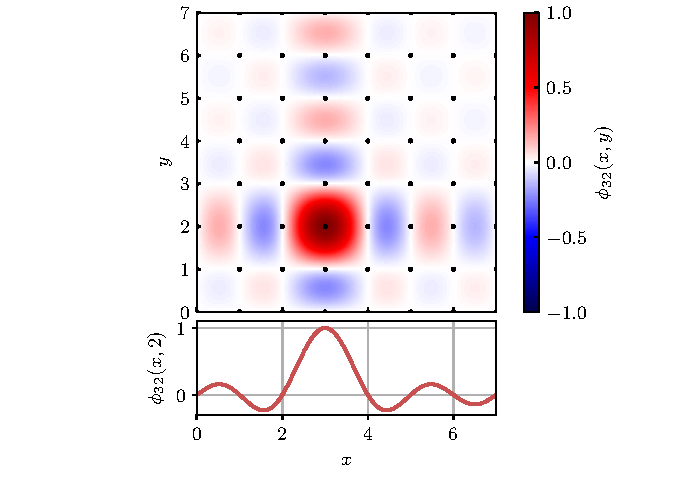
\includegraphics[width=\textwidth]{figures/numerics/basis_vecs.pdf}
    \caption{[basis vecs]}
    \label{fig:basis_vecs}
\end{figure}

The spatial representation of the basis vectors $\{\ket{\vec r_{ij}}\}$ can be computed using \eqref{eq:spatial_plane_wave_basis} as:
\begin{align}
\phi_{ij}(\vec r) &= \braket{\vec r}{\vec r_{i j}} = \sum_{i^\prime j^\prime} e^{-\ii \vec k_{i^\prime j^\prime} \cdot \vec r_{i j}}\braket{\vec r}{\vec k_{i^\prime j^\prime}}\\
\Rightarrow \phi_{ij}(\vec r) &=\begin{cases}
\sum_{i^\prime j^\prime} \frac 1 {\sqrt A} e^{\ii \vec k_{i^\prime j^\prime} \cdot (\vec r - \vec r_{i j})}\qquad (\vec r\ \textrm{within \textsc{2d} region})\\
0\qquad(\vec r\ \textrm{not within \textsc{2d} region}),
\end{cases}
\end{align}
and an example is plotted in \figref{fig:basis_vecs}.

These functions are sometimes called \emph{periodic sinc functions}, or \emph{band-limited delta functions} [CITE]. Each of them is zero at all of the gridpoints except one, and and they form an orthonormal basis set. They satisfy all of our requirements to be a basis corresponding to our gridded discretisation of space. Thus, the approach of discretising space on a grid is indeed equivalent to choosing a (necessarily incomplete) orthonormal basis in which to work.

One thing to note is that these functions are periodic. By using the Fourier basis in the way we have to restrict our basis to cover only a finite region of both Fourier space and real space, we have necessarily imposed periodicity on the problem. This periodicity shows itself when we compute matrix elements of operators in this basis - if we compute the kinetic energy operator's matrix elements for example, it will couple basis states across the boundary of the region, resulting in spatial periodicity---a wavepacket moving rightward through the right boundary will emerge moving rightward from the left boundary.

Perhaps less obviously, the basis is also periodic in Fourier space, and so a wavepacket moving out of the region of Fourier space simulated will also wrap around to the opposite side of Fourier space. In real space, this may appear as a wavepacket undergoing acceleration only to suddenly reverse its velocity as if reflected off a barrier. This effect is entirely unphysical\footnote{With the possible exception of the region of Fourier space being simulated corresponding to the first Brillouin zone of a lattice potential, in which case these velocity reversals would correspond to Bloch oscillations.} and should be taken as a sign that the spatial grid is not fine enough for the dynamics being simulated.

The discrete Fourier basis we've described is one example of a \emph{spectral basis}, and a numerical method which represented the state vector solely in this basis would be called a \emph{spectral method}. Other choices of basis functions, such as polynomials ([SECREF FEDVR]) or harmonic oscillator basis functions ([SECREF]) lead one to other spectral methods. Perhaps surprisingly, the corresponding discrete spatial basis discussed above, despite being related to the Fourier basis by a unitary transformation, is instead called a \emph{pseudospectral} basis, and a method representing the state vector in this basis a \emph{pseudospectral method}. Although it is ``just another basis", the fact that the basis functions are zero at all spatial points bar one each leads to the possibility of a further approximation when representing some operators, which makes bases with this property especially useful. I describe this in the following section.

\subsubsection{Vector and matrix elements in the Fourier and pseudospectral bases}

We now have a finite basis $\{\ket{\vec r_{ij}}\}$ that matches our intuitions somewhat for representing a wavefunction at a set of gridpoints. A state vector can be approximated as a linear sum of these basis vectors, with the coefficient for each one being equal to the projection of state vector's wavefunction onto the basis vector's wavefunction:
\begin{align}\label{eq:vector_elements_pseudospectral}
\ket{\psi} \approx \sum_{ij} \psi_{ij} \ket{\vec r_{i j}},
\end{align}
where
\begin{align}
\psi_{i j} = \int \phi_{ij}^*(\vec r) \psi(\vec r) \dd{\vec r}.
\end{align}
In practice however this integral is rarely done. Instead, $\psi_{ij}$ is simply taken to be the value of the exact wavefunction $\psi(\vec r) = \braket{\vec r}{\psi}$ at the point $\vec r = \vec r_{ij}$:
\begin{align}\label{eq:pseudospectral_vector}
\psi_{i j} \approx \psi(\vec r_{ij})
\end{align}
 To see why this is a good approximation, imagine that the approximation \eqref{eq:vector_elements_pseudospectral} were exact, that is, $\psi(\vec r)$ were exactly equal to a linear sum of the functions $\{\phi_{ij}(\vec r)\}$. Since all the basis functions are zero at the point $\vec r_{ij}$ except for $\phi_{ij}$, the value of $\psi(\vec r_{ij})$ must come solely from the $\psi(\vec r)$'s projection onto the basis function $\phi_{ij}(r)$. Since approximating \eqref{eq:vector_elements_pseudospectral} underlies the results of any simulation that discretises a state vector in this way, treating it as exact for the initial projection onto the discrete basis is making an assumption no worse than that already being relied upon.


With a basis and initial discrete state vector in hand, we can now proceed to calculate matrix elements of the Hamiltonian, after which we can proceed to solve the differential equation \eqref{eq:schrodinger_equation_matrix_vector} to determine how the coefficients $\{\psi_{ij}\}$ evolve in time.

The specific properties of our Fourier/pseudospectral basis make it quite useful for a range of common Hamiltonians. For example, let's take the single particle Schr\"odinger Hamiltonian:
\begin{align}
\hat H_\textrm{Schr\"o} = \frac{\hbar^2 \hat k ^2}{2m}  + V(\hat {\vec r}),
\end{align}
where $\hat k = |\hat{\vec k}|$.

The two terms, kinetic and potential, are each diagonal in different bases. The kinetic term is diagonal in the Fourier basis:

\begin{align}
\matrixel{\vec k^\prime}{\frac{\hbar^2 \hat k^2}{2m}}{\vec k} = \frac{\hbar^2 k^2}{2m}\delta(\vec k - \vec k^\prime),
\end{align}
where $k = |\vec k|$, and the potential term is diagonal in the spatial basis:
\begin{align}
\matrixel{\vec r^\prime}{V(\hat{\vec r})}{\vec r} = V(\vec r) \delta(\vec r - \vec r^\prime).
\end{align}
The kinetic term is also diagonal our discrete Fourier basis:
\begin{align}
K_{\up{Fourier}, i^\prime j^\prime i j} = \matrixel{\vec k_{i^\prime j^\prime}}{\frac{\hbar^2 \hat k^2}{2m}}{\vec k_{i j}} = \frac{\hbar^2 k_{i j}^2}{2m}\delta_{i^\prime i}\delta_{j^\prime j},
\end{align}
however---perhaps surprisingly---the potential term is not diagonal in the pseudospectral basis, only approximately so:
\begin{align}\label{eq:pseudospectral_operator}
V_{\up{real}, i^\prime j^\prime i j} = \matrixel{\vec r_{i^\prime j^\prime}}{V(\hat{\vec r})}{\vec r_{i j}} \approx V(\vec r_{i j}) \delta_{i^\prime i}\delta_{j^\prime j}.
\end{align}
Nonetheless, equation \eqref{eq:pseudospectral_operator} is in practice treated as exact for the purpose of computing matrix elements in the discrete basis of operators that are diagonal in the full spatial basis. As above with projecting a state vector using simply the values of a wavefunction at the gridpoints (rather than doing integrals), treating this approximation as exact is equivalent to making the assumption that the potential $V(\vec r)$ is already accurately representable in the discrete basis as a diagonal operator:
\begin{align}
V(\vec r) \approx \sum_{ij} V(\vec r_{ij}) \phi^\ast_{ij}(\vec r)\phi_{ij}(\vec r),
\end{align}
and so similarly is going to be a good approximation whenever the discrete basis is well able to represent the potential. So long as your discrete basis can accurately represent the state vectors and spatially-diagonal operators you will be using, it makes little difference whether you project those vectors and operators onto the basis using integrals or using simply their values at the gridpoints.

This alternate method of projection has a name, it is called \emph{collocation}\cite[p227]{tannor_introduction_2007}. Using collocation instead of vector projection amounts to treating our basis vectors as a scheme for interpolating state vectors and operators in between gridpoints, given their values at the points, rather than as basis vectors to project upon. Another way to interpret collocation is to say that we are evaluating the vector projections using integrals after all, however, we're numerically computing those integrals using a quadrature scheme, only evaluating the integrand at the gridpoints and performing a discrete sum\cite[p283]{tannor_introduction_2007}. Collocation is what puts the \emph{pseudo} in pseudospectral---if we evaluated all these operators using integrals instead, we would be treating the discrete spatial basis exactly the same as any spectral basis. 

Compared to a purely spectral method, pseudospectral methods are of comparable accuracy\cite{orszag_comparison_1972}. This makes intuitive sense---discrete sums instead of integrals is how we are going to do all inner products once we are in the discrete basis---so it can't be much worse to use the same method to approximate operators and initial state vectors. The sole downside of pseudospectral methods, according to \cite{orszag_comparison_1972}, is that the error can lead to instability in the presence of certain nonlinearities. Specifically, if long wavelength waves interact in a way that would produce wavelengths shorter than two grid spacings (the Nyquist wavelength), pseudospectral methods will produce longer wavelength waves instead, whereas in a purely spectral method the interaction would not occur, being due to couplings to a Fourier mode outside the discrete Fourier basis. This \emph{aliasing} can cause instability, but can be circumvented with smoothing techniques \cite{phillips_example_1959}. This is no great downside: if you want to simulate short length scales, you need to choose a grid spacing small enough to represent them, whereas if short wavelengths are produced despite your willingness to ignore them, you must smooth them away before they are aliased into long wavelengths that you do care about.

Finally, armed with a kinetic energy operator in Fourier space and a pseudospectral approximation to the potential operator in real space, we can write all the matrix elements of $\hat H_\textrm{Schr\"o}$ in a single basis, and thus our discretised, pseudospectral two-dimensional Schr\"odinger wave equation:
\begin{align}
\ii\hbar\dv{t}\psi_{i^\prime j^\prime}(t) &= \sum_{ij} H_{i^\prime j^\prime, ij}(t) \psi_{ij}(t)\\
\Rightarrow \ii\hbar\dv{t}\psi_{i^\prime j^\prime}(t) &=\sum_{ij}
\left[
U^\dagger_{\textsc{dft2}}K_\up{Fourier}U_{\textsc{dft2}}
 + V_\up{real}(t)
\right]_{i^\prime j^\prime, ij}\psi_{ij}(t),
\end{align}
where we have used the discrete Fourier transform to transform the kinetic energy operator into the discrete real space basis, and allowed the potential operator to be possibly time dependent.

The right hand side of this expression can now simply be evaluated, yielding the time derivative of each component $\psi_{ij}(t)$ of the discrete state vector $\vec\psi(t)$:
\begin{align}\label{eq:discrete_de_matrices}
\dv{t}\vec\psi(t) &= -\frac{\ii}{\hbar} \left[U^\dagger_{\textsc{dft2}}K_\up{Fourier}U_{\textsc{dft2}}\vec\psi(t) + V_\up{real}(t)\vec\psi(t)\right]\\
\Rightarrow \dv{t}\vec\psi(t) &= -\frac{\ii}{\hbar} \left[
\fft_2^{-1}\left\{\frac{\hbar^2 \tilde{\vec k}^{\odot2}}{2m}\odot\fft_2\left\{\vec\psi(t)\right\}\right\}
+ V(\tilde{\vec r}, t)\odot\vec\psi(t)\right],\label{eq:discrete_fft_de}
\end{align}
where $\fft_2$ is the two dimensional fast Fourier transform, an efficient implementation of the discrete Fourier transform (taking time $\Ord{n \log n}$ in the size of each dimension), $\tilde{\vec r}$ is a vector (of vectors) containing each discrete position vector (such that $V(\tilde{\vec r}, t)$ is a vector (of scalars) containing the potential evaluated at each discrete position), $\tilde{\vec k}$ is a vector (of vectors) containing each discrete $k$-vector, such that $\tilde{\vec k}^{\odot2}$ is a vector (of scalars) containing the squared magnitude of each discrete $k$-vector, and 
$\odot$ represents elementwise multiplication (or exponentiation) of vectors. Other than $\vec \psi$, these vectors are more akin to arrays used in programming languages than to members of a vector space, hence the somewhat clunky notation in \eqref{eq:discrete_fft_de}. Comparison with the continuous version of equation \eqref{eq:discrete_fft_de} (i.e. the Schr\"odinger wave equation \eqref{eq:schrodinger_wave_equation}), since elementwise multiplication of functions is a more common operation in mathematics, might be clarifying:
\begin{align}
\pdv{t}\psi(\vec r, t) &= -\frac{\ii}{\hbar} \left[
\mathcal{F}^{-1}\left\{
\frac{\hbar^2 k^2}{2m}\mathcal{F}\left\{\psi(\vec r, t)\right\}(\vec k)
\right\}(\vec r)
+ V(\vec r, t)\psi(\vec r, t)
\right],
\end{align}
where $\mathcal{F}$ is the continuous Fourier transform, and $k$ as always is $\abs{\vec k}$. So we see that the discretised Schr\"odinger equation for a single particle in a potential really is the same as evaluating the continuous equation at a set of gridpoints, evaluating spatial derivatives in Fourier space, and replacing the continuous Fourier transform with its discrete equivalent.

Here is an example of how one might compute the \textsc{rhs} of \eqref{eq:discrete_fft_de} in Python code:

\python{code_listings/dpsi_dt_fourier.py}

Where the example is for a time-independent potential. If the potential were time dependent, \texttt{V\_real} within the function \texttt{dpsi\_dt(t, psi)} would need to be replaced with a call to a function that returned an array for \texttt{V\_real} at time \texttt{t}.

Starting with some initial discrete wavefunction, this could then be solved with a forward differencing scheme like fourth order Runge--Kutta (section \ref{sec:rk4}):

\python{code_listings/rk4.py}

The discretised differential equation \eqref{eq:discrete_de_matrices} can also be solved using a split-step method (section \ref{sec:split-step}), since the Hamiltonian matches the requirements of being written as a sum of terms for which individually an eigenbasis is known (the discrete real space basis for the potential term, and the Fourier basis for the kinetic term). For example, here is how one might implement second or fourth-order split-step (only a single timestep shown):

\python{code_listings/fourier_split_step.py}

In all the above code examples, a nonlinear term as in the case of the Gross-Pitaevskii equation can be included in the potential simply by adding a term \texttt{g * np.abs(psi)**2} to the potential \texttt{V\_real} wherever it appears. As discussed in section \ref{sec:limitations_nonlinearity}, the nonlinearity poses no problem for the split-step methods so long as the potential term of the Hamiltonian is evaluated as the outermost sandwich of exponentials in the second-order split step method (which comprises the sub-steps of fourth-order split-step).

\subsection{Finite differences}
Fourier split-step, or using discrete Fourier transforms to evaluate the spatial derivatives at each gridpoint in order to time-evolve using Runge--Kutta are effective and versatile numerical methods.

The use of discrete Fourier transforms in the previous section can be seen as replacing the Laplacian operator in the Schr\"odinger wave equation \eqref{eq:schrodinger_wave_equation} with the equivalent operation in Fourier space:
\begin{align}\label{eq:dft_laplacian}
\nabla^2\psi(\tilde{\vec r}) \approx \fft_2^{-1}\left\{-\tilde{\vec k}^{\odot 2} \odot \fft_2\left\{\psi(\tilde{\vec r})\right\}\right\},
\end{align}
where as before $\tilde{\vec r}$ is a vector (of vectors) containing the discrete positions, $\vec{\tilde k}$ is a vector (of vectors) containing discrete $k$-vectors such that $\vec{\tilde k}^{\odot 2}$ is a vector (of scalars) containing the squared magnitudes of each $k$-vector, and $\odot$ represents elementwise multiplication or exponentiation of vectors. More generally for any derivative,
\begin{align}\label{eq:dft_derivative}
\pdv{x}\psi(\tilde{\vec r}) \approx \fft_2^{-1}\left\{\ii\tilde{\vec k}_x \odot \fft_2\left\{\psi(\tilde{\vec r})\right\}\right\},
\end{align}
where $\tilde{\vec k}_x$ is a vector (of scalars) containing the discrete angular wavenumbers for the $x$ spatial dimension.

Equations \eqref{eq:dft_laplacian} and \eqref{eq:dft_derivative} are exact for any wavefunction $\psi(\vec r)$ which is periodic and band-limited to the discrete Fourier space (and thus exactly representable as a vector $\vec \psi$ of its values at each gridpoint), which is why the Fourier method of computing derivatives this way is sometimes said to be accurate to ``infinite order" [CITE] in the grid spacings $\upDelta x$ and $\upDelta y$, in contrast to fixed-order approximations to derivatives which are second, fourth, sixth order etc. In practice the Fourier method for derivatives is often used for wavefunctions which are \emph{not} intended to be periodic (the periodicity imposed by using the method is unphysical), and so for these it has merely very high order accuracy, not literally infinite. 

In any case, such high accuracy is not often necessary---if one is using only an $\Ord{\upDelta t^4}$ accurate timestepping scheme, then the timestepping may be the limiting factor in overall accuracy and it might be wise to decrease the accuracy of computing spatial derivatives if there is otherwise a benefit to doing so.

To that end, the Fourier method of derivatives may be replaced with \emph{finite differences} instead. Although finite differences are usually derived as approximations to derivatives directly from the definition of the derivative without reference to discrete Fourier transforms, they can be considered fixed-order approximations to the Fourier method \cite{fornberg_pseudospectral_1987}. Thus operators whose form in Fourier space corresponds to a derivative of some order can be approximated with finite differences:
\begin{align}
U^\dagger_{\textsc{dft2}} k_x U_{\textsc{dft2}}\psi(\tilde{\vec r}) = 
-\ii\delta^{(n)}_{\upDelta x} \otimes \mathbb{I}_{n_y}\psi(\tilde{\vec r}) + \Ord{\upDelta x^n}
\end{align} 
where $k_x$ is the diagonal matrix of the discrete angular wavenumbers for the $x$ spatial dimension and $\delta^{(n)}_{\upDelta x}$ is the matrix representing $n^\up{th}$ order finite difference approximation to the first derivative using grid spacing $\upDelta x$. The matrix elements of this and some other central finite differences are shown in \tableref{table:fd_matrixels}.

\begin{table}\label{table:fd_matrixels}
\centering
\begin{tabular}[c]{|r||rrrrrrr|}
\hline
 & $k=-3$ & $k=-2$ & $k=-1$ & $k=0$ & $k=1$ & $k=2$ & $k=3$\\
\hline
$\upDelta x\left(\delta^{(2)}_{\upDelta x}\right)_{i, i+k}$ 
& & & $-\frac{1}{2}$ & $0$ & $\frac{1}{2}$ & & \\
$\upDelta x\left(\delta^{(4)}_{\upDelta x}\right)_{i, i+k}$ 
& & $\frac{1}{12}$ & $-\frac{2}{3}$ & $0$ & $\frac{2}{3}$ & $-\frac{1}{12}$ & \\
$\upDelta x\left(\delta^{(6)}_{\upDelta x}\right)_{i, i+k}$ 
& $-\frac{1}{60}$ & $\frac{3}{20}$ & $-\frac{3}{4}$ & $0$ & $\frac{3}{4}$ & $-\frac{3}{20}$ & $\frac{1}{60}$\\
$\upDelta x^2\left(\delta^{2 (2)}_{\upDelta x}\right)_{i, i+k}$ 
& & & $1$ & $-2$ & $1$ & & \\
$\upDelta x^2\left(\delta^{2 (4)}_{\upDelta x}\right)_{i, i+k}$ 
& & $-\frac{1}{12}$ & $\frac{4}{3}$ & $-\frac{5}{2}$ & $\frac{4}{3}$ & $-\frac{1}{12}$ & \\
$\upDelta x^2\left(\delta^{2 (6)}_{\upDelta x}\right)_{i, i+k}$ 
& $\frac{1}{90}$ & $-\frac{3}{20}$ & $\frac{3}{2}$ & $-\frac{49}{18}$ & $\frac{3}{2}$ & $-\frac{3}{20}$ & $\frac{1}{90}$\\
\hline
\end{tabular}
\caption{Matrix elements \cite{fornberg_generation_1988} for some finite-differencing schemes for first ($\delta^{(n)}_{\upDelta x}$) and second ($\delta^{2 (n)}_{\upDelta x}$) derivatives using central finite differences of various orders $n$ for uniform grid spacing $\upDelta x$. All finite difference matrices are banded; each column here shows the matrix elements of $k^\up{th}$ diagonal, which are all identical. Elements outside of each matrix's band are left blank. Each matrix element is shown multiplied by factors of $\upDelta x$ for clarity.}
\end{table}

The fact that the finite difference matrices are banded allows them to be computing by applying a ``stencil" to a discrete state vector, computing an approximation to some linear sum of derivative operators at each point of discrete space by consideration of only that point and a small number of surrounding point. For example, a $\Ord{\upDelta x^2}$ approximation (assuming $\upDelta x = \upDelta y$) to the kinetic energy operator in two dimensions may be evaluated at each point as:
\begin{align}
K_\up{real}\psi(\tilde{\vec r}) & = U^\dagger_{\textsc{dft2}} \frac{\hbar^2 (k_x^2 + k_y^2)}{2m} U_{\textsc{dft2}}\psi(\tilde{\vec r})\label{eq:2DKreal}\\
&= -\frac{\hbar^2}{2m} \left[
  \delta^{2 (n)}_{\upDelta x} \otimes \mathbb{I}_{n_y}
+ \mathbb{I}_{n_x} \otimes \delta^{2 (2)}_{\upDelta y}\right]\psi(\tilde{\vec r}) + \Ord{\upDelta x^2}\label{eq:finite_differences_subspaces}
\end{align} 
\begin{align}
\Rightarrow \left(K_\up{real}\psi(\tilde{\vec r})\right)_{ij}
= -\frac{\hbar^2}{2m} &\left[ - 4\psi(x_i,  y_j)
                             + \psi(x_{i-1},  y_j) + \psi(x_{i+1},  y_j) \right.\nonumber\\
                            &\left.  + \psi(x_i,  y_{j-1}) + \psi(x_i,  y_{j+1})\right] + \Ord{\upDelta x^2}.
\end{align} 

Thus the kinetic energy operator, when approximated using finite differences, is an example of an operator that can be written as a sum of banded operators acting on different subspaces of the total Hilbert space---the identity matrices in \eqref{eq:finite_differences_subspaces} each leave a part of the Hilbert space untouched. As mentioned in [SECREF], this in principle considerably reduces the computational cost of applying the approximate kinetic energy operator to a discretised state vector. Fourier transforms, when computed with the fast Fourier transform algorithm, are already less computationally expensive than a general matrix-vector multiplication, that is, the fast Fourier transform allows one to multiply the matrix $U_{\textsc{dft2}}$ in \eqref{eq:2DKreal} by a vector considerably faster than $\Ord{n_x^2n_y^2}$, which would be the computational time-complexity for a general $n_xn_y \times n_xn_y$ matrix. Firstly, a two-dimensional discrete Fourier transform can also be written as the sum of two one-dimensional transformations operating on different subspaces:
\begin{align}
U_{\textsc{dft2}} =
U_{\textsc{dft},x} \otimes \mathbb{I}_{n_y} + \mathbb{I}_{n_x} \otimes U_{\textsc{dft},y},
\end{align}
where $U_{\textsc{dft},x}$ and $U_{\textsc{dft},y}$ are the unitaries for one-dimensional discrete Fourier transforms in the $x$ and $y$ dimensions respectively. So even if $U_{\textsc{dft},x}$ and $U_{\textsc{dft},y}$ were arbitrary matrices, this already would reduce the cost of multiplying $U_{\textsc{dft2}}$ by a vector to $\Ord{n_y n_x^2 + n_x n_y^2}$ But they are not arbitrary matrices---each of these one-dimensional Fourier transforms has computational cost $\Ord{n \log n}$ using the \textsc{fft} algorithm, where $n$ is the number of points in the relevant dimension, resulting in an overall cost of $\Ord{n_y n_x \log n_x + n_x n_y\log n_y}$ for applying the two-dimensional Fourier transform $U_{\textsc{dft2}}$ to a vector. Finite differences improves on this further. As discussed in [SECREF], since our finite-differences approximation to the kinetic energy operator can written as the sum of banded matrices operating on different subspaces, the computational cost of applying it to a vector is $\Ord{bn_xn_y}$, where $b$ is the bandwidth of the banded matrices, which depends on which order accuracy is used (for example, for second order finite-differences $b=1$). This is faster than the Fourier method of computing the kinetic energy operator by a factor of $\Ord{\log n_x + \log n_y}$. Whilst this seems considerable, the difference is hard to observe in pracice. On ordinary computers the number of points needs to be increased so much in order to measure any difference in speed between the algorithms that the data no longer fits in \textsc{cpu} cache and copying the data to and from main memory becomes the bottleneck. Although copying data from memory is a linear-time process, the coefficient of that linear time is large enough to make the asymptotic speed of finite differences vs. Fourier transforms not relevant for ordinary computers, in my experience.

No, the practical advantages of finite differences compared to Fourier transforms do not come down to single-core speed. Rather, they are:
\begin{enumerate}
    \item Being banded matrices, the finite-difference approximations to the kinetic energy operator can be multiplied by a vector, or exponentiated and applied to a vector, in parallel on a cluster computer or \textsc{gpu} using the techniques discussed in section [SECREF], whereas the fast Fourier transform is less efficiently parallelisable \cite{Gupta93thescalability}. The speed of finite differences can have very nice scaling with the number of \textsc{cpu} cores or cluster nodes used, since only $b$ points need to be exchanged between cores at each step when applying or exponentiating the kinetic energy operator. For large problems, `superscaling' can even be observed, whereby the speedup factor obtained by moving to multiple \textsc{cpu}s or compute nodes on a cluster is larger than the number of \textsc{cpu}s/nodes used. This is counterintuitive, but comes from more effectively using \textsc{cpu} cache---by spreading the data over multiple cores, one minimises the proportion of the state vector that needs to reside in main memory instead of in (much faster) \textsc{cpu} cache at any one time.
    \item One can intervene at the boundaries to impose boundary conditions other than periodicity. Strictly speaking, as an approximation to the Fourier method of computing derivatives, the indices for the matrix elements as given in \tableref{table:fd_matrixels} should be read as wrapping around to the other side of the spatial region whenever they would go out of bounds---that is, $(\delta^{2 (n)}_{\upDelta x})_{i, i + k}$ should be read as $(\delta^{2 (n)}_{\upDelta x})_{i, (i + k) \mod n_x}$. However, as mentioned, periodicity is often an undesired consequence of the Fourier method of derivatives. Alternatively one can simply omit these matrix elements that would couple spatial points across the boundary, which has the result of imposing zero boundary conditions instead of periodic. Judicious deletion of matrix elements at other points in space can also be used to impose zero boundary conditions elsewhere, equivalent to an infinite potential barrier which would otherwise be numerically troublesome if done with the potential energy term of the Hamiltonian. Other interventions in the application of the kinetic energy operator can be used to impose other boundary conditions such as constant-value, constant-gradient, etc., whereas the Fourier method is less flexible in this respect.
    \item Finite differences are compatible with non-uniform grids, whereas the Fourier method is limited to uniform grids. Non-uniform grids imply different matrix elements \cite{fornberg_generation_1988} for the finite difference operators, but are otherwise treated exactly the same. This allows more dense placement of gridpoints in regions where wavefunctions may have finer spatial structure, without having to waste computational power on regions of space where the wavefunction is known to have only coarser structure. An example is an electron in a Coulomb potential, an accurate simulation of which would need to capture fine details at small radii but less detail at larger radii. A transformation into spherical coordinates with a non-uniform grid for the radial coordinate could be well treated with finite differences.
    \item Finite differences are compatible with the use of split-step methods with some operators that are diagonal in neither Fourier nor real space. For example, the real-space representation of the operator for the $z$ component of angular momentum is $L_z = -\ii\hbar\left(x\pdv{y} - y \pdv{x}\right)$. With diagonal matrices $X$ and $Y$ being used for the the $\hat x$ and $\hat y$ operators in accordance with the pseudospectral method, and finite differences being used to approximate the derivatives, the result is a banded matrix representation of $L_z$, compatible with the techniques from section [SECREF parallel] for reducing the problem to that of many small matrices instead of one big one. There is a little more complexity, $L_z$ cannot be represented as a sum of operators acting on the $x$ and $y$ subspaces separately---instead, each term in $L_z$ is a \emph{product} of operators that act on different subspaces. Consider the first term of a discretised version of $L_z$ using fourth-order finite differences. It can be diagonalised in the following way:
    \begin{align}
        -\ii\hbar X \otimes \delta^{(4)}_{\upDelta y}
        = -\ii\hbar\left(\mathbb{I}_{n_x} X \mathbb{I}_{n_x}\right)
        \otimes \left(Q_{\delta_y}^\dagger D_{\delta_y}Q_{\delta_y}\right),
    \end{align}
    where $Q_{\delta_y}$ and $D_{\delta_y}$ are the unitary and diagonal matrix that diagonalise $\delta^{(4)}_{\upDelta y}$ ($X$ is already diagonal, and so is `diagonalised' by the identity matrix for the $x$ subspace). $\mathbb{I}_{n_x}$ and $X$ act on the $x$ subspace, whereas $Q_{\delta_y}$ and $D_{\delta_y}$ act on the $y$ subspace, and since matrices operating on different subspaces commute, this can be rearranged to:
    \begin{align}\label{eq:Lz_split}
        -\ii\hbar X \otimes \delta^{(4)}_{\upDelta y}
        = \left(\mathbb{I}_{n_x} \otimes Q_{\delta_y}^\dagger\right)
        \left(-\ii\hbar X \otimes  D_{\delta_y}\right)
        \left(\mathbb{I}_{n_x} \otimes Q_{\delta_y}\right),
    \end{align}
yielding a diagonalisation of the original matrix that can be used to apply an exponentiation of the original matrix to a vector with matrix-vector multiplications only in the $x$ any $y$ subspaces and not the total Hilbert space. Here, the matrix-vector multiplication in the $x$ subspace is the identity, but more generally the above idea can be used to exponentiate any operator that can be written as the product of operators that act on different subspaces:
\begin{align}\label{eq:arb_product_operators}
e^{A \otimes B} =
\left(Q^\dagger_A \otimes Q^\dagger_B\right)
e^{\left(D_A \otimes D_B\right)}
\left(Q_A \otimes Q_B\right).
\end{align}
Since $X$ is already diagonal, $\delta^{(4)}_{\upDelta y}$ can be written as the sum of two block-diagonal matrices as described in [SECREF PARALLEL], allowing \eqref{eq:Lz_split} to be evaluated as the sum of two terms $-\ii\hbar X \otimes \delta^{(4)}_{\upDelta y} = -\ii\hbar (X \otimes \delta_\up{even} + X \otimes \delta_\up{odd})$, one for each of the block-diagonal matrices $\delta_\up{even}$ and $\delta_\up{odd}$. The diagonalisation of each term then has matrix-vector products taking place in a space of the size of each block, that is, in the expression
\begin{align}
-\ii\hbar X \otimes \delta_\up{even} = \left(\mathbb{I}_{n_x} \otimes Q_\up{even}^\dagger\right)
        \left(-\ii\hbar X \otimes  D_\up{even}\right)
        \left(\mathbb{I}_{n_x} \otimes Q_\up{even}\right),
\end{align}
the unitary $Q_\up{even}$ is also block-diagonal. This splitting allows for parallel application of the exponentiation of $L_z$ to a vector as well as speeding up single-core computation on account of the smaller matrices, as described in section [SECREF].

However If a matrix that were not diagonal were present instead of $X$, such as another derivative operator, then if we wanted to split \emph{both} matrices each into a sum of two block-diagonal matrices, equation \eqref{eq:arb_product_operators} would become \emph{four} terms rather than two, and the flow of data for a parallel computation would be somewhat more complicated. For a term in the Hamiltonian that is a product of $n$ operators acting on different subspaces, the number of terms obtained by splitting them all in this way grows exponentially with $n$. But, when all but one operator in the product is diagonal already, as is the case for angular momentum operators, then splitting can be done as normal.

\end{enumerate}

To conclude this section, there are clear advantages to using finite differences as opposed to Fourier transforms when it comes to parallelisability, boundary conditions, and non-uniform grids, but if these are not a concern then both Fourier transforms and finite differences run at approximately equal speeds in practice, meaning one should use whichever is easiest to implement.

Many of these advantages of finite differences over Fourier methods are also enjoyed by the finite element discrete variable representation (\textsc{fedvr}) method, discussed in the next section. Whilst it's also claimed that \textsc{fedvr} has a number of advantages over finite-differences [CITE PRE], I'll argue that most of the comparisons don't stand up to scrutiny, and that finite differences are often still the right choice for the contexts in which \textsc{fedvr} is argued to be superior.

\subsection{The finite element discrete variable representation}

Another method of spatial discretisation is the finite element discrete variable representation (\textsc{FEDVR}) [CITE]. As the name suggests, it is a finite element method, with a set of basis functions in each element, and each element linked at their boundaries. Here I will not go into detail about the \textsc{fedvr} method, more detail can be found in [THE TEXTBOOK] and specifically in the context of Bose-Einstein condensation, [THOSE TWO PAPERS ABOUT IT]. I'll instead introduce the points that are relevant to the conclusion that I drew regarding the method for the purposes of time-evolving wavefunctions, which is that it is not particularly compared to simple central finite differences.

As a finite element method, \textsc{FEDVR} divides space into a number of `elements', joined to their neighbouring elements at their edges, within which the function being solved for is represented as a sum of basis functions. Finite element methods such as this are useful for problems with irregular boundary conditions, or requiring variable grid sizes, as the elements need not have the same size (area/volume, etc) as each other, and parameters on which the accuracy of the numerical method depends can be varied from element to element, such that precision is high where it is needed and low where it is not. In addition, the basis functions used within the elements can be chosen so that conserved properties of the differential equation are also inherently conserved by the simulation resulting in a \emph{geometric integrator}. The \textsc{fedvr} method though does not make use of this possibility, although it can be used with split-step methods for time propagation, which preserve the wavefunction's norm.

Within each element in the \textsc{fedvr} method, the wavefunction is represented as a linear sum of a set of polynomial basis functions, specially chosen to have some desirable properties. The polynomials are not orthogonal, but at a set of gridpoints, all but one of them is zero, meaning that as with the Fourier pseudospectral method, they can be used as a pseudospectral basis --- computing how much of each polynomial to include in the representation of a wavefunction by using only the wavefunction's value at the gridpoint at which each polynomial is zero, and computing the matrix elements of operators using approximate integration based on a discrete sum taking into account only those same gridpoints.

So far (within each element at least) what I have described does not sound too different to the Fourier pseudospectral method. And it would be not different at all if the gridpoints were equally spaced, if one allowed the number of points to go to infinity, and one used the lowest order polynomials that were each zero at all points but one. But in the discrete variable representation --- which is what the method used within each element of \textsc{frdvr} is called when used by itself --- the gridpoints are not equally spaced. Rather they are more densely packed toward the edges of the element, and least densely packed in the middle of each element. The locations of the gridpoints are chosen according to a \emph{quadrature rule}, which is a method of approximate the definite integral of a function as a  weighted sum of the function's values at a specific set of points. There are many quadrature rules, each with a different set of points and weights, but a common feature to them is that the points are more closely spaced at the edges of the integration region. In the context of the pseudospectral method, the chosen quadrature rule is what we are using when we are evaluating integrals based only on the function's values at discrete points. For equally spaced points, the weights are all equal, but for unequally spaced points they are not (and vary depending on the quadrature rule in use).

The use of unequally spaced points increases the accuracy of integrals evaluated this way. One would think that equally spaced points would produce the most accurate approximate integrals, but this is not true for finite regions, or systems without periodic boundary conditions, due to the presence of a boundary. For finite, non-periodic regions, approximating functions as polynomials equal to the value of the function at a discrete set of points is vulnerable to Runge's phenomenon --- spurious oscillations in the approximation near the edges of the region [CITE]. The oscillations are minimised, however, if the density of points increases near the edge, specifically if the density of points approaches $1/\sqrt{1 - x^2}$ for the normalised integraiton region $x \in [-1, 1]$ as the number of points goes to infinity [CITE - REFERENCE AVAILABLE ON WIKIPEDIA RUNGE'S PHENOMONENON] (see Figure [FIGREF]). 

[FIGURE OF POLYNOMIAL INTERPOLATION EQUAL AND UNEQUAL OF GAUSSIAN]

By choosing a quadrature scheme with two points located exactly on each edge of the integration regions, such as \emph{Gauss-Lobatto} quadrature [CITE], the elements of the \textsc{fedvr} method can be joined together, with adjacent elements sharing these edge points (see figure [FIGREF]). This allows one to represent a wavefunction as a list of coefficients for how much of each basis polynomial in each element contributes to it, with the extra condition that some of these coefficients --- those corresponding to the edge points --- must be equal in order to ensure the wavefunction is continuous across the boundaries between elements.

\begin{figure}[t]
    \centerfloat
    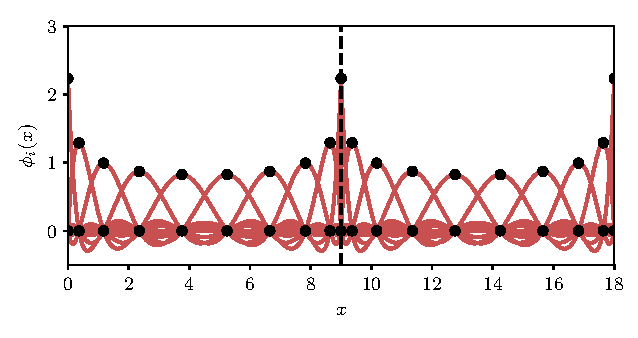
\includegraphics{figures/numerics/fedvr_basis.pdf}
    \caption{CAPTION}
    \label{fig:fedvr_basis}
\end{figure}

With some care taken in regard to the points shared between the elements, the \textsc{fedvr} method provides one with a means of approximating wavefunctions as a finite sum of basis functions, and of approximately calculating the matrix elements of operators in this basis. After that, one can simply apply the operators to the state vectors in order to compute time derivatives, and propagate in time using fourth order Runge--Kutta or similar [SEE SECREF], or one can exponentiate the operators, all at once or one at a time, as part of a split-step method [SEC SECREF]. The \textsc{FEDVR} method does not require anything in particular about time propagation --- like finite differences or the Fourier pseudospectral method, it is only a way of spatially discretising the differential equation you are trying to solve.

Now we arrive at what makes the \textsc{FEDVR} method exciting for those who want to massively parallelise their simulations. When one calculates the matrix representation of, say, a one-dimensional differential operator in the \textsc{fedvr} basis, one gets matrices that look like \figref{fig:fedvr_D2_operator}.

\begin{figure}[t]
    \centerfloat
    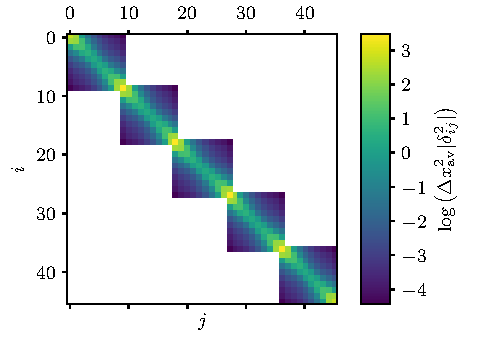
\includegraphics{figures/numerics/fedvr_D2_operator.pdf}
    \caption{The matrix form of the second derivative operator in \textsc{fedvr}, for 5 elements each with ten \textsc{dvr} points. The colour scale is logarithmic, showing the log of the absolute values of the matrix elements $\delta^2_{ij}$ scaled by $\upDelta x_\up{av}^2$, where $\upDelta x_\up{av}$ is the average spacing between the unequally spaced grid points. Zero matrix elements are shown as white. One can see that the second derivative at each grid point is computed using only the points within the same element, except for one point shared by adjacent elements, at which the second derivative depends on points in both adjacent elements.}
    \label{fig:fedvr_D2_operator}
\end{figure}

With this almost-block-diagonal form. This is because when the state vector is acted upon by some operator, the result for most points in the resulting vector depends only on the points in the input vector \emph{within the same element}. The exceptions are the points shared between elements---for which the value in the output vector depends on the points in the input vector in \emph{both} adjacent elements, which is why the matrix is not perfectly block diagonal.

Why is this exciting? Well, it means that the operator can be written like this:

[SUM OF MATRICES]

Which is very similar to the splitting of finite-difference matrices in section [SECREF], and in the same way allows the matrix or its exponentiation to be efficiently applied to a state vector in parallel. The difference between this and the finite differences case is the number of points of overlap between the two matrices, which corresponds to the amount of data that must be transferred between parallel threads or cluster nodes during a parallel computation. In finite differences, the number of points that must be exchanged at boundaries in each step or sub-step of whichever time propagation method is used is equal to the bandwidth of the matrix. In \textsc{fedvr}, so long as the boundaries of the regions of space assigned to each thread or cluster node aligns with the border between two elements, \emph{only one} point must be exchanged. Increasing the number of points within each element - but reducing the number of elements so as to keep the total number of points constant, decreases the discretisation error of the method, but still, only one point needs to be exchanged at boundaries. Whereas with finite differences, increasing the order of the finite difference scheme requires more points to be exchanged at the boundaries. So it would seem that \textsc{fedvr} ought to scale much better in parallel implementations, which is a large part of its appeal [CITE].

However, I've noticed that when using both \textsc{fedvr} and finite differences to simulate Bose--Einstein condensates using the Gross--Pitaevskii equation, smaller timesteps are required when using the \textsc{fedvr} method [SHOULD I SHOW THIS EXPLICITLY?] in otherwise comparable setups. By this I mean that, without damping, the error of the \textsc{gpe} simulated using \textsc{rk4} (which is a conditionally stable algorithm), there is a timestep size at which the simulation is unstable and diverges. Similarly in split-step methods, although the error is bounded, there is a timestep size at which the error rapidly grows to that bound and the wavefunction no longer even approximately resembles the true solution. Below this threshold timestep, the error scales as $\Ord{\upDelta t^4}$ for \textsc{rk4}, and $\Ord{\upDelta t^4}$, $\Ord{\upDelta t^2}$, $\Ord{\upDelta t}$ for fourth, second, and first order split-step respectively, as expected. But in practice, all these methods are so accurate that one desires to use the largest timestep one can without this blowup (or soft-blowup in the case of the unitary split-step methods) occurring during the time interval one wants to simulate. And my observation was that the threshold timestep is always smaller for \textsc{fedvr} than for finite differences or the Fourier method for determining spatial derivatives, necessitating smaller timesteps for stability or the same degree of pseudo-stability.

So why is this? For \textsc{rk4}, what is the stability critereon and why might \textsc{fedvr} violate it mkore easily than finite differences? And how might we understand the sudden decrease in accuracy of the split-step methods at a similar threshold timestep size, despite them being unconditionally stable?

The stability critereon for \textsc{rk4} when applied to a linear differential equation of the form:

\begin{align}
\dv{\vec\psi}{t} = A\vec\psi,
\end{align}
where A is a matrix with all imaginary eigenvalues (as is the case for Hamiltonian evolution where $A=-\frac \ii \hbar H$), is\cite{caplan_numerical_2011-1}:
\begin{align}
\upDelta t < \frac{2 \sqrt 2}{|\lambda|_\up {max}}
\end{align}
where $|\lambda|_\up {max}$ is the absolute value of the largest (by absolute value) eigenvalue of $A$.

The Gross--Pitaevskii equation is not linear, but we'll put that to the side for the moment---it will be relevant shortly. In the linear case of the Schr\"odinger wave equation, the maximum absolute value of $A$'s eigenvalues will be the maximum absolute eigenvalue from the kinetic term, plus the maximum absolute eigenvalue from the potential term. Using the Fourier pseudospectral method to compute spatial derivatives, the largest eigenvalue of the kinetic part of the Hamiltonian is that of the Nyquist mode with $k_\up{Nyquist} = \pi / \upDelta x$ for grid spacing $\upDelta x$, and this is approximately true of finite differences as well, leading to:
\begin{align}
|\lambda|_\up {max} &\approx \Abs{-\frac \ii \hbar \frac{\hbar^2 k_\up{Nyquist}}{2m}}
+ \Abs{-\frac \ii \hbar V(\vec r)}_\up{max}\\
\Rightarrow \upDelta t &\lessapprox \frac{2\sqrt 2 \hbar}
{\frac{\hbar^2\pi^2}{2m \upDelta x^2} + \abs{V(\vec r)}_\up{max}}.
\end{align}
In the limit of small $\upDelta x$, the kinetic term dominates and the stability criterion becomes:
\begin{align}
\upDelta t &\lessapprox \frac{4\sqrt 2 m \upDelta x^2}{\pi^2 \hbar},
\end{align}
whereas in the limit of large potential:
\begin{align}
\upDelta t &\lessapprox \frac{2\sqrt 2\hbar}{\abs{V(\vec r)}_\up{max}}.
\end{align}
These results match our intuition somewhat in terms of dynamical phase evolution---eigenvalues of the Hamiltonian are energies and determine how quickly the elements of the state vector accumulate dynamical phase. For each circle around the complex plane that a dynamical phase of $2\pi$ entails, we expect to require at least a few timesteps to resolve said circle, and the above shows that 'a few' means at least $2\sqrt{2}$.

As a sidenote, if it is known which term of the Hamiltonian dominates the stability criterion, that term can be removed by use of an \emph{interaction picture} [CITE, SECREF?], essentially treating the dynamical phase evolution due to that term analytically. And if the term is not constant, but is \emph{almost} constant, one can still treat \emph{most} of the dynamical phase evolution analytically, transforming the differential equation onto one with much smaller eigenvalues for that term, in both cases allowing one to take potentially much larger timesteps due to the above reasoning. Fourth order Runge--Kutta in the interaction picture (\textsc{rk4ip}) [CITE] uses an interaction picture to treat the kinetic term of the Schr\"odinger or Gross--Pitaevskii equation analytically, whereas my `fourth order Runge--Kutta in an instantaneous, local interaction picture' method presented in section [SECREF] removes (most of) the potential term. Both methods allow larger timesteps to be taken, but in different circumstances depending on which term is dominating the Hamiltonian.

The problem with \textsc{fedvr} then, is that it requires smaller timesteps than finite differences because its kinetic energy operator has larger eigenvalues than an equally accurate finite difference method. How much larger?

[POSSIBLY MOVE THIS ARGUMENT TO EARLIER IN THIS SECTION]

In order to make a fair comparison, we need to know how many \textsc{dvr} basis functions are required per element in order to compute equally accurate second derivatives as a given finite difference scheme. With $N$ points per element, \textsc{fedvr} represents the state vector within each element in a spectral basis of polynomials up to degree $N - 1$. Therefore a polynomial of degree $N - 1$ or less can be represented exactly, any other function is subject to truncation error. If one varies the number of points per element, varying the number of elements in order to keep the total number of points constant, the truncation error in representing an arbitrary function in this basis is therefore $\Ord{\upDelta x^N}$, where $\upDelta x$ is either the size of each element, or equivalently the average spacing between grid points (these two differing only by a constant factor if the total number of points is held constant).

In \textsc{fedvr} the derivative operator, regardless of whether its matrix elements are computed with integrals or the quadrature rule, is exact \cite{schneider_discrete_2005}. The relevant error in a derivative of a wavefunction is therefore determined by this truncation error of representing it in the spectral basis in the first place:

\begin{align}
\psi_\up{approx}(x_i) = \psi_\up{exact}(x_i) + \Ord{\upDelta x^N}\\
\Rightarrow\psi^{\prime \prime}_\up{approx}(x_i) =  \psi^{\prime\prime}_\up{exact}(x_i) + \Ord{\upDelta x^{N-2}}.
\end{align} 

Central finite difference approximations to second derivatives on the other hand have error $\Ord{\upDelta x^{N - 1}}$ where N is the total number of points used to compute the derivative at each point (for example the 3-point central finite difference rule for second derivatives has error $\Ord{\upDelta x^2}$, the 5 point rule is accurate to $\Ord{\upDelta x^4}$, etc). With this knowledge we can translate our question

\begin{quote}
Which is less computationally intensive to simulate the \textsc{gpe} or Schr\"odinger wave equation: $m^\up{th}$-order accurate \textsc{fedvr} or $m^\up{th}$-order accurate finite differences?
\end{quote}
to
\begin{quote}
which is less computationally intensive to simulate the \textsc{gpe} or Schr\"odinger wave equation: $m+2$ points-per-element \textsc{fedvr} or $m+1$ point central finite differences?
\end{quote}
The argument in favour of \textsc{fedvr} is that as $m$ grows, finite differences require an increasing number of points to be exchanged at the boundaries between cluster nodes/threads etc in a parallel implementation, whereas so long as the border between spatial regions allocated to different cluster nodes aligns with the border between elements, only one point need be exchanged per timestep in \textsc{fedvr}, no matter how many points per element there are. Therefore, in the limit of high accuracy, \textsc{fedvr} wins.

The problem with this argument is that it compares only the amount of work that needs to be done \emph{per timestep}. But, since the allowed timestep size required for stability (at least for fourth order Runge--Kutta, I'll argue shortly why I think this generalises to other timestepping schemes as well) depends on the maximum eigenvalues of the kinetic energy operator, and the kinetic energy operator is not the same as $m$ grows, more work is needed to show which method is least computationally expensive per unit \emph{simulation time}.

The maximum eigenvalue of the kinetic energy operator when approximated using central finite differences does not change appreciably as the number of points used to compute derivatives increases --- indeed, the eigenspectrum converges to that of the Fourier method [CITE], with maximum eigenvalue equal to the kinetic energy of the Nyquist mode. The kinetic energy operator approximated with \textsc{fedvr} on the other hand does not have an approximately constant maximum eigenvalue as one increases the number of points per element whilst holding the total number of gridpoints constant [SEE FIG]

\begin{figure}[t]
    \centerfloat
    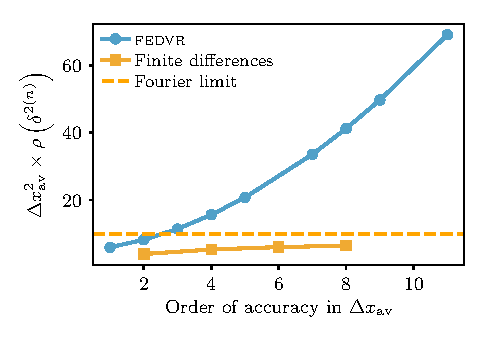
\includegraphics{figures/numerics/fedvr_eigenvalue_scaling.pdf}
    \caption{Scaling of maximum (by absolute value) eigenvalue of second derivative operator with respect to the order of accuracy for finite differences and \textsc{fedvr}. Results were numerically computed by constructing a $721\times721$ matrix (chosen to allow various combinations of number of \textsc{dvr} points per element whilst holding total points constant) for each point and numerically diagonalising. The largest eigenvalue for \textsc{fedvr} can be seen to scale quadratically with the order of accuracy, whereas for finite differences the maximum eigenvalue approaches that of the Fourier method.}
    \label{fig:fedvr_eigenvalue_scaling}
\end{figure}

First in order to make a fair comparison, we need to know how many \textsc{dvr} basis functions are required per element in order to compute equally accurate second derivatives as a given finite difference scheme. Gauss--Lobatto quadrature with $N$ points can compute an integral exactly if the integrand is a polynomial of degree $2N - 2$ or less \cite{schneider_discrete_2005}---This means that the error in evaluating an integral using the quadrature rule is $\Ord{\upDelta x^{2N - 1}}$ where $\upDelta x$ is the size of the element. If one has a fixed number of points overall, but is varying the number of points per element (varying the number of elements to keep the number of points in total approximately fixed), then the $\upDelta x$ in the integration error $\Ord{\upDelta x^{2N - 1}}$ can equivalently be considered to be the average spacing between points, which differs from the width of an element in this case by a constant factor. This will be useful for making fair comparisons to finite differences.

Having $N$ points, the basis functions of $N$-points-per-element \textsc{fedvr} basis are polynomials of order $N - 1$. This means that the integrand

The origin of this maximum timestep is the minimum spatial grid size $\upDelta x_\up {min}$. Although the rigorous result is shown with proper stability analysis, the heuristic reasoning goes like this: one can ask, what is the fastest speed that information can propagate in my system? Approximating that the kinetic term of the \textsc{gpe} dominates the dispersion relation, for a uniform grid this speed will be the group velocity of the Nyquist mode, which has wavelength $2\upDelta x$. More generally for a nonuniform grid it will be the same velocity but for the fastest `local' Nyquist mode with wavelength $2\upDelta x_\up {min}$ where $\upDelta x_\up {min}$ is the smallest grid spacing present. The dispersion relation then gives us the group velocity of this mode:

\begin{equation}
v_\up{g}(k_\up{Nyquist}) = \pdv{E_\up{K}(k_\up{Nyquist})}{p(k_\up{Nyquist})} =  \frac{\pi \hbar}{m \upDelta x_\up{min}}
\end{equation}

Then one can compute how long it takes for a pulse moving at this speed to propagate over the shortest distance $\upDelta x_\up{min}$, yielding the `dispersion timescale':
\begin{equation}
\tau_\up d = \frac{m\upDelta x_\up{min}^2 }{\pi \hbar}
\end{equation} 

This timescale answers the question ``What is the longest interval of time for which you can be guaranteed that no feature of the wavefunction has moved further than the smallest grid spacing?". This sets an upper limit for the timesteps that can be used to simulate the Gross--Pitaevskii equation regardless of which of the spatial or temporal discretisation schemes described so far is used. For linear differential equations this may not be true, since linear waves can pass through each other unaffected, but with the Gross--Pitaevsii equation's nonlinearity, one can see that if the nonlinear term is not evaluated at intervals at least as short as $\tau_\up d$, then it cannot be taking into account density fluctuations due to interference between high wavenumber modes, leading to inaccuracy. The higher the wavenumber of possible nodes, the shorter the timesteps must be to capture all their dynamics.

\begin{figure}[t]
    \centerfloat
    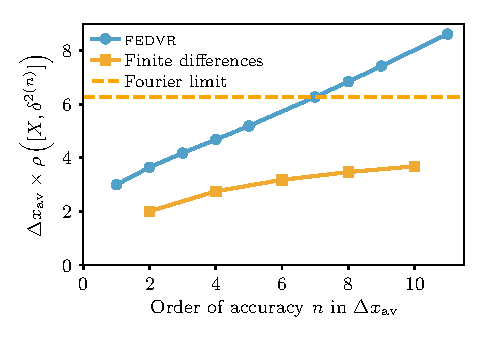
\includegraphics{figures/numerics/fedvr_commutation_error_scaling.pdf}
    \caption{TODO CAPTION once mentioned in text about unitary methods}
\end{figure}


\begin{itemize}
    \item Summarise, don't go into detail. Just a different method of spatial discretisation.
    \item{Splits space into `elements'. Briefly mention what these are good for - funky boundary conditions and irregular grids mostly}
    \item Represents state vector within each element using interpolating polynomials - they're a basis but they're not an orthonormal one. Each one is zero all points in each element except one. To get coefficients in this basis you get the wavefunction's values at the specific points in space (you can't just do a projection, because the basis isn't orthonormal - you'd get a state vector with >1 norm if you did that). To reconstruct a wavefunction again you sum the interpolating polynomials with their coefficients.
    \item Benefit of finite elements in general, other than boundary conditions and variable grids is that you can choose basis functions within elements that conserve some known conserved quantities, and hence you can make geometric integrators.
    \item Differential operators can be computed using the quadrature rule, and then you can solve using Runge-Kutta or split-step. The main paper on all this [CITE] uses fourth order split-step.
    \item For the Schrodinger and Schrodinger-like equations, purported benefit other than irregular gridding and boundary conditions is that you only need to exchange one point between elements, speeding up parallel implementations.
    \item Go into why that actually doesn't help:
    \item Conceptually I like to think of DVR as non-central finite differences on an irregular grid. Finite differences are also based on interpolating polynomials. Central finite differences of say, 6th order accuracy would require sending four points across compute-node boundaries every time you want to apply an operator to a state vector. But, non-central finite differences within individual elements, instead of central finite differences everywhere, can make it such that within elements, points need every other point in order to compute a differential operator - but they only require one point across element boundaries. The differential operators are still same order accuracy in $\updelta x$. But, now they're subject to Gibbs'/Runge's phenomenon. So, you solve this by making the points unequally spaced. [Such and such theorem] says that you optimally supress the oscillations near the element boundaries if the point spacing scales like [however it scales]. So you space the points unevenly like that, recompute your differential operators based on what the interpolating polynomials now look like, and you have a DVR basis. If you force points to be on element boundaries and do some tricks to join elements together, you now have an FEDVR basis.
    \item The paper compares 6th order [and other order] FEDVR to 2nd order finite differences for accuracy in representing the 2D SHO groundstate. FEDVR wins the comparison. But, i think it's not a fair comparison becuse they only used second order central finite differences. 6th order central finite differences are just as accurate as 6th order FEDVR.
    \item But if you use 6th order central finite differences, you have to pass 4x more points at compute-node boundaries compared to FEDVR. So that means FEDVR parallelises better, right? Wrong. Not for time-evolution, and not for the Schrodinger equation. Maximum timestep you can take (regardless of RK or split-step) is set by the kinetic term and is intuitive - you can't take timesteps longer than the time it takes the fastest mode to move the smallest frid spacing.
    \item FEDVR has \emph{smaller minimum grid spacing}. It requires smaller timesteps. How much smaller? [SHOW CALCULATION] Enough to mean that you have to take 16x as many timesteps compared to FD. So you thought you were sending four times less data compared to central finite differences, but you're actually sending four times more, because you are only sending four times less per timestep - and you are taking sixteen times as many timesteps.

    \item So unless you're using it in order to have irregular grids or strange boundary conditions, FEDVR provides little benefit for time-evolving Schrodinger-like equations. Finite differences can be used on irregular grids too [CITE]

\end{itemize}

\subsection{Harmonic oscillator basis functions}

[Another way of discretising space. Not a grid at all. Useful in, well, harmonic and approximately harmonic potentials, or (well, equivalently) when Hamiltonian is sparse in the SHO eigenbasis. Otherwise not great - without FFTs, applying the Hamiltonian means big, dense matrices - slow.]



    % \subsection{Unitary integration}
    %     \subsubsection{Direct exponentiation via diagonalisation of Hamiltonian}
    %     \begin{itemize}
    %     \item Unitary - doesn't mean it's accurate but means it won't explode. Great for the bits of your simulation that are explosion-prone but don't matter (like regions of space where the wavefunction is near zero but the potential is large or steep)
    %     \item error is order [whatever it is] per timestep, not great compared to RK4
    %     \item can be combined with RK4 to improve accuracy (see later subsection)
    %     \end{itemize}
    %     \subsubsection{Approximate exponentiation by operator product}

    %     [Comment in this section how the approximate total unitary can be used at each timestep to define an interaction picture, and the remaining dynamics simulated with RK4 like RKILIP does in the spatial basis. Interaction pictures are really useful!]

% \section{Continuous degrees of freedom}



%     Every symbol on the paper has a representation in a computer. State vectors are arrays of complex numbers, operators are matrices - differential operators are no exception. Operators must have a concrete representation, their matrix elements can be computed and then things solved with linear algebra. For discrete degrees of freedom, the matrix representation of the operators may be known, for continuous ones you can find the matrix elements once you define what basis functions you will use [show how]. Or, for the DVR it is a little more subtle (because it's not a basis) but still basically the same process.

%     \begin{itemize}
%         \item Have to be discretised in some way to simulate on a computer - need basis functions. Often a spatial basis is used. Any spatial basis must be combined with assumptions about what the wavefunction is doing at points in between the basis points, in order to define differential operators. Finite differences approximates wavefunction as low-order polynomial in between points (is this equivalent to a polynomial \emph{basis}? Probably not.). Fourier method assume the Fourier series of the wavefunction at the given points can be used to interpolate between points (or the wavefuntion can be Fourier transformed and calculations can be done directly in the Fourier basis). DVR is not actually a spatial basis despite appearances. It assumes the wavefunction is a sum of polynomial 'shape functions', but these shape functions are not basis functions as they are not orthonormal. This is why it is called a representation rather than a basis. Regardless, the shape functions can be used to define an interpolation of the wavefunction between points and thus define differential operators.

    % \end{itemize}
    % \subsection{Finite differences}
    %     Show a matrix representation of a few different finite differences, to show that differential operators really are just matrices. They approximate the function as low-order polynomials about each point. You can take them to arbitrarily high order.
    % \subsection{The Fourier basis}
    %     Because of properties of Fourier transforms, derivitives can be taken in Fourier space as simple multiplication. This is essentially because differential operators are diagonal in the Fourier basis. So you can use this fact to define a differential operator in the spatial basis [show matrix] ...or, you could just implement it with Fourier transforms, since FFTs are faster than matrix-vector multiplication ($O(n \log (n)$) rather than $O(n^2)$)
    %     \subsubsection{Split operator method}
    %         \begin{itemize}
    %         \item Equivalent to approximate exponentiation via operator product with the discrete case
    %         \end{itemize}

\section{Finding ground states}
\subsection{Imaginary time evolution}
[Summarise ITEM]
\subsection{Successive over-relaxation}
[Summarise SOR]
\subsection{Generalisation to excited states via Gram–Schmidt orthonormalisation}
Directly diagonalising a Hamiltonian can be costly in a spatial basis. Another approach is to find the ground state using one of the above techniques, and then repeat the process, subtracting off the wavefunction's projection onto the already found ground state at every step. This yields the lowest energy state that is orthogonal to the first - i.e. the first excited state. Repeating the process, but subtracting off \emph{both} eigenstates found so far, then yields the second excited state and so forth. This is simply the Gram-Schmidt process for finding orthonormal vectors, with the additional step of relaxing each vector to the lowest possible energy for each one - this ensures the eigenstates of the Hamiltonian are produced, rather than a different orthogonal basis. Extra conditions can be imposed on the wavefunction at each relaxation step in order to obtain particular solutions in the case of degenerate eigenstates. For example, a phase winding can be imposed in order to obtain a particular harmonic oscillator state - otherwise this process produces an arbitrary superposition of basis states that have equal energy.

% \section{The finite-element discrete variable representation}

% - Plots of representation of sine wave as function of number of points between FEDVR and FD. RMS error of a derivative operator perhaps.

% [explanation of how it works, comparison of implementation with RSP4 vs something like RK4. RK4 is more general purpose, method does not need to be modified for different Hamiltonians. Main limitation is inability to factor out fast dynamical phases, see RK4ILIP for solution to this. MPI implementation and scaling properties with increasing cores. Superscaling at low number of cores. Mention how my implementation can tolerate high network latency due to early sending od data before all local computations are complete. Mention that it is ripe for GPU processing. Limitations: vulnerable to Runge's phenomenon for sharp potentials. Can't increase the order of the polynomials much because small spacing at the edges requires tiny timesteps. Possible solution: pre-conditioning the potential to be an approximation better representable in the DVR basis.]

% \endinput % Remove once numerics completed

\section{Fourth order Runge--Kutta in an instantaneous local interaction picture}\label{sec:rk4ilip}

\sectionmark{RK4 in an instantaneous local interaction picture}

Consider the differential equation for the components of a state vector $\ket{\psi(t)}$ in a particular basis with basis vectors $\ket{n}$. This might simply be the Schr\"odinger equation, or perhaps some sort of nonlinear or other approximate, effective or phenomenological equation not corresponding to pure Hamiltonian evolution. Though they may have additional terms, such equations are generally of the form:
\begin{align}\label{eq:schrodinger_eq}
\dv t \braket{n}{\psi(t)} = -\frac i \hbar \sum_m \matrixel{n}{\hat H(t)}{m} \braket{m}{\psi(t)},
\end{align}
where $\matrixel{n}{\hat H(t)}{m}$ are the matrix elements in that basis of the Hamiltonian $\hat H(t)$, which in general can be time dependent, or even a function of $\ket{\psi(t)}$, depending on the exact type of equation in use. If $\hat H(t)$ is almost diagonal in the $\ket{n}$ basis, then the solution to \eqref{eq:schrodinger_eq} is dominated by simple dynamical phase evolution, that is:
\begin{align}
\ket{\psi(t)} \approx \sum_m e^{-\frac i \hbar E_m t}\ket{m},
\end{align}
where $E_m$ is the energy eigenvalue corresponding to the eigenstate $\ket{m}$.

A transformation into an interaction picture (\textsc{ip}) \cite[p318]{sakurai} is commonly used to treat this part of the evolution analytically, before solving the remaining dynamics with further analytics or numerics. For numerical methods, integration in the interaction picture allows one to use larger integration timesteps, as one does not need to resolve the fast oscillations around the complex plane due to this dynamical phase.

Choosing an interaction picture typically involves diagonalising the time-independent part of a Hamiltonian, and then proceeding in the basis in which that time-independent part is diagonal. However, often one has a good reason to perform computations in a different basis, in which the time independent part of the Hamiltonian is only approximately diagonal,\footnote{For example, a spatial basis which allows for partitioning the integration region over multiple nodes on a cluster or cores on a \textsc{gpu}.} and transforming between bases may be computationally expensive (involving large matrix-vector multiplications). Furthermore, the Hamiltonian may change sufficiently during the time interval being simulated that the original time-independent Hamiltonian no longer dominates the dynamics at later times. In both these cases it would still be useful to factor out the time-local oscillatory dynamics in whichever basis is being used, in order to avoid taking unreasonably small timesteps.

To that end, suppose we decompose $\hat H(t)$ into diagonal and non-diagonal (in the $\ket{n}$ basis) parts at each moment in time:
\begin{align}
\hat H(t) = \hat H_\up{diag}(t) + \hat H_\up{nondiag}(t),
\end{align}
and use the diagonal part at a specific time $t=t^\prime$ to define a time-independent Hamiltonian:
\begin{align}\label{eq:H0def}
 \hat H_0^{t^\prime} = \hat H_\up{diag}(t^\prime),
\end{align}
which is diagonal in the $\ket{n}$ basis. We can then use then use $\hat H_0^{t^\prime}$ to define an interaction picture state vector:
\begin{align}\label{eq:IP_definition}
\ket{\psi_\up{I}^{t^\prime}(t)} = e^{\frac i \hbar (t - t^\prime) \hat H_0^{t^\prime}}\ket{\psi(t)},
\end{align}
which obeys the differential equation:
\begin{align}\label{eq:IPDE}
\dv t \ket{\psi_\up{I}^{t^\prime}(t)}
    = e^{\frac i \hbar (t - t^\prime) \hat H_0^{t^\prime}}\dv t \ket{\psi(t)}
      + \frac i\hbar \hat H_0^{t^\prime}\ket{\psi_\up{I}^{t^\prime}(t)},
\end{align}
where:
\begin{align}\label{eq:backtransform}
\ket{\psi(t)} = e^{-\frac i \hbar (t - t^\prime) \hat H_0^{t^\prime}}\ket{\psi_\up{I}^{t^\prime}(t)}
\end{align}
is the original Schrödinger picture (\textsc{sp}) state vector.

This transformation is exact, no approximations or assumptions have been made. If indeed the dynamics of $\ket{\psi(t)}$ in the given basis are dominated by fast oscillating dynamical phases, that is, the diagonals of $\hat H_\up{diag}(t)$ are much greater than all matrix elements of $\hat H_\up{nondiag}(t)$ in the $\ket{n}$ basis, then solving the differential equation \eqref{eq:IPDE} for $\ket{\psi_\up{I}^{t^\prime}(t)}$ should allow one to use larger integration timesteps than solving \eqref{eq:schrodinger_eq} directly. And if not, then it should do no harm other than the (small) computational costs of computing some extra scalar exponentials.

Equation \eqref{eq:IP_definition} defines an \emph{instantaneous} interaction picture, in that it depends on the dynamics at a specific time $t=t^\prime$, and can be recomputed repeatedly throughout a computation in order to factor out the fast dynamical phase evolution even as the oscillation rates change over time. It is \emph{local} in that $H_0^{t^\prime}$ is diagonal in the $\ket{n}$ basis, which means that transformations between Schrödinger picture and interaction picture state vectors involves ordinary, elementwise exponentiation of vectors, rather than matrix products. Thus \eqref{eq:IP_definition}, \eqref{eq:IPDE} and \eqref{eq:backtransform} can be written componentwise as:

\begin{align}\label{eq:IP_definition_components}
\braket{n}{\psi_\up{I}^{t^\prime}(t)} = e^{ i (t - t^\prime)\omega_n^{t^\prime}}\braket{n}{\psi(t)},
\end{align}
\begin{align}\label{eq:IPDE_components}
\dv t \braket{n}{\psi_\up{I}^{t^\prime}(t)}
    = e^{i (t - t^\prime)\omega_n^{t^\prime}}\dv t \braket{n}{\psi(t)}
      + i\omega_n^{t^\prime}\braket{n}{\psi_\up{I}^{t^\prime}(t)},
\end{align}
and:
\begin{align}\label{eq:backtransform_components}
\braket{n}{\psi(t)} = e^{-i(t - t^\prime)\omega_n^{t^\prime}}\braket{n}{\psi_\up{I}^{t^\prime}(t)},
\end{align}
where we have defined:
\begin{align}\label{eq:omega}
\omega_n^{t^\prime} = \frac 1\hbar \matrixel{n}{\hat H_0^{t^\prime}}{n}
\end{align}
This is in contrast to fourth order Runge--Kutta in the interaction picture (\textsc{rk4ip}) \cite{caradoc_davies_thesis}, in which the interaction picture uses the Fourier basis and thus transforming to and from it involves fast Fourier transforms (\textsc{fft}s). \textsc{rk4ip} was developed to augment computations in which \textsc{fft}s were already in use for evaluating spatial derivatives, and so its use of \textsc{fft}s imposes no additional cost. Nonetheless, an interaction picture based on the kinetic term of the Schr\"odinger equation (which is the term of the Hamiltonian that \textsc{rk4ip} takes as its time-independent part) may not be useful if that term does not dominate the Hamiltonian, as in the case of a Bose--Einstein condensate in the Thomas--Fermi limit. We compare the two methods below.

\subsection{Algorithm}
The \emph{fourth order Runge--Kutta in an instantaneous local interaction picture} \textsc{rk4ilip} algorithm is now obtained by using \eqref{eq:IP_definition} to define a new interaction picture at the beginning of each fourth-order Runge–Kutta (\textsc{rk4}) integration timestep. The differential equation and initial conditions supplied to the algorithm are in the ordinary Schr\"odinger picture, and the interaction picture is used only within a timestep, with the Schrödinger picture state vector returned at the end of each timestep. Thus differential equations need not be modified compared to if ordinary \textsc{rk4} were being used, and the only modification to calling code required is for a function to compute and return $\omega_n^{t^\prime}$.

Being based on fourth order Runge--Kutta integration, this new method enjoys all the benefits of a workhorse method that is time-proven, and---as evidenced by its extremely widespread use---at a sweet-spot of ease of implementation, accuracy, and required computing power \cite{artofscientificcomputing1992}.

Below is the resulting algorithm for performing one integration timestep. It takes as input the time $t_0$ at the start of the timestep, the timestep size $\upDelta t$, an array $\mathbf{\psi}_0$ containing the components $\{\braket{n}{\psi(t_0)}\}$ of the state vector at time $t_0$, a function $F(t, \mathbf{\psi})$ which takes a time and (the components of) a state vector and returns an array containing the time derivative of each component, and a function $G(t, \mathbf{\psi})$ which takes the same inputs and returns an array containing the interaction picture oscillation frequency $\omega_n$ for each component at that time.

For example, for the case of the Gross--Pitaevskii equation \cite{pethick2002bose} in the spatial basis $\psi(\vec r, t) = \braket{\vec r}{\psi(t)}$, these would be:
\begin{align}\label{eq:RK4_ILIP_GPE}
F(t, \psi(\vec r, t)) &= -\frac i \hbar\Bigg[\underbrace{-\frac{\hbar^2}{2m}\nabla^2}_{\hat H_\up{nondiag}} + \underbrace{V(\vec r, t) + g|\psi(\vec r, t)|^2}_{\hat H_\up{diag}}\Bigg]\psi(\vec r, t),
\end{align}
and
\begin{align}
G(t, \psi(\vec r, t)) = \frac1\hbar\big[\underbrace{V(\vec r, t) + g|\psi(\vec r, t)|^2}_{\hat H_\up{diag}}\big].
\end{align}

Note that each symbol in bold in the algorithm below denotes an array containing one element for each basis vector $\ket{n}$, subscripts denote the different stages of \textsc{rk4}, and all arithmetic operations between arrays are elementwise\footnote{For example, the expression \mbox{$\mathbf{a}\leftarrow e^{-i\mathbf{\omega}\upDelta t}\mathbf{b}$} indicates that for all $n$, \mbox{$a_n\leftarrow e^{-i\omega_n\upDelta t}b_n$}, where $a_n$ denotes the $n^\up{th}$ element of $\mathbf{a}$ etc.} The only opportunity for non-elementwise operations to occur is within $F$, which contains the details (via $\hat H_\up{nondiag}$) of any couplings between basis states for whatever system of equations is being solved, for example, using \textsc{fft}s or finite differences to evaluate the Laplacian in \eqref{eq:RK4_ILIP_GPE}.


\begin{breakablealgorithm}
    \caption{\textsc{rk4ilip}}
    \begin{algorithmic}[1]
    \linespread{1.5}
    \footnotesize
    \Function{$\up{RK4ILIP}$}{$t_0$, $\upDelta t$, $\mathbf{\psi}_0$, $F$}
        \State $\mathbf{f}_1 \gets F(t_0, \mathbf{\psi}_0)$
        \Comment{First evaluation of Schrödinger picture DE}
        \State $\mathbf{\omega} \gets G(t_0, \mathbf{\psi}_0)$
        \Comment{Oscillation frequencies: $\hbar\omega_n = \matrixel{n}{\hat H_\up{diag}(t_0)}{n}$}
        \State $\mathbf{k}_1 \gets \mathbf{f}_1 + i\mathbf{\omega}\mathbf{\psi}_0$
        \Comment{Evaluate \eqref{eq:IPDE_components} with $t-t^\prime=0$}
        \State $\mathbf{\phi}_1 \gets \mathbf{\psi}_0 + \mathbf{k}_1 \frac{\upDelta t}{2}$
        \Comment{First RK4 estimate of IP state vector, at $t=t_0 + \frac{\upDelta t}{2}$}
        \State $\mathbf{\psi}_1 \gets e^{-i\mathbf{\omega}\frac{\upDelta t}{2}}\mathbf{\phi}_1$
        \Comment{Convert first estimate back to SP with \eqref{eq:backtransform_components}}
        \State $\mathbf{f}_2 \gets F(t_0 + \frac{\upDelta t}{2}, \mathbf{\psi}_1)$
        \Comment{Second evaluation of Schrödinger picture DE}
        \State $\mathbf{k}_2 \gets e^{i\mathbf{\omega}\frac{\upDelta t}{2}}\mathbf{f}_2 + i\mathbf{\omega}\mathbf{\phi}_1$
        \Comment{Evaluate \eqref{eq:IPDE_components} with $t-t^\prime=\frac{\upDelta t}{2}$}
        \State $\mathbf{\phi}_2 \gets \mathbf{\psi}_0 + \mathbf{k}_2 \frac{\upDelta t}{2}$
        \Comment{Second RK4 estimate of IP state vector, at $t=t_0 + \frac{\upDelta t}{2}$}
        \State $\mathbf{\psi}_2 \gets e^{-i\mathbf{\omega}\frac{\upDelta t}{2}}\mathbf{\phi}_2$
        \Comment{Convert second estimate back to SP with \eqref{eq:backtransform_components}}
        \State $\mathbf{f}_3 \gets F(t_0 + \frac{\upDelta t}{2}, \mathbf{\psi}_2)$
        \Comment{Third evaluation of Schrödinger picture DE}
        \State $\mathbf{k}_3 \gets e^{i\mathbf{\omega}\frac{\upDelta t}{2}}\mathbf{f}_3 + i\mathbf{\omega}\mathbf{\phi}_2$
        \Comment{Evaluate \eqref{eq:IPDE_components} with $t-t^\prime=\frac{\upDelta t}{2}$}
        \State $\mathbf{\phi}_3 \gets \mathbf{\psi}_0 + \mathbf{k}_3 \upDelta t$
        \Comment{Third RK4 estimate of IP state vector, at $t=t_0 + \upDelta t$}
        \State $\mathbf{\psi}_3 \gets e^{-i\mathbf{\omega}\upDelta t}\mathbf{\phi}_3$
        \Comment{Convert third estimate back to SP with \eqref{eq:backtransform_components}}
        \State $\mathbf{f}_4 \gets F(t_0 + \upDelta t, \mathbf{\psi}_3)$
        \Comment{Fourth evaluation of Schrödinger picture DE}
        \State $\mathbf{k}_4 \gets e^{i\mathbf{\omega}\upDelta t}\mathbf{f}_4 + i\mathbf{\omega}\mathbf{\phi}_3$
        \Comment{Evaluate \eqref{eq:IPDE_components} with $t-t^\prime=\upDelta t$}
        \State $\mathbf{\phi}_4 \gets
                \mathbf{\psi}_0 + \frac{\upDelta t}{6}\left(\mathbf{k}_1 + 2\mathbf{k}_2 + 2\mathbf{k}_3 + \mathbf{k}_4\right)$
        \Comment{Fourth RK4 estimate, at $t=t_0 + \upDelta t$}
        \State $\mathbf{\psi}_4 \gets e^{-i\mathbf{\omega}\upDelta t}\mathbf{\phi}_4$
        \Comment{Convert fourth estimate back to SP with \eqref{eq:backtransform_components}}
        \State \Return $\mathbf{\psi}_4$
        \Comment{Return the computed SP state vector at $t=t_0 + \upDelta t$}
    \EndFunction
    \end{algorithmic}
\end{breakablealgorithm}

\subsubsection{Note on imaginary time evolution}

When \textsc{rk4ilip} is used for imaginary time evolution (\textsc{ite}) \cite{chiofalo2000}, the oscillation frequencies $\mathbf{\omega}$ may have a large imaginary part. If the initial guess is different enough from the ground state, then the exponentials in \eqref{eq:IP_definition_components}, \eqref{eq:IPDE_components} and \eqref{eq:backtransform_components} may result in numerical overflow. To prevent this, one can define a clipped copy of $\mathbf{\omega}$,
\begin{align}
\mathbf{\omega}_\up{clipped} = \re(\mathbf{\omega}) + i\begin{cases}
-\frac{\log X}{\upDelta t}\qquad \im(\mathbf{\omega})\upDelta t < -\log X\\
\im(\mathbf{\omega})\qquad       -\log X \leq \im(\mathbf{\omega})\upDelta t \leq \log X\\
\frac{\log X}{\upDelta t}\qquad  \im(\mathbf{\omega})\upDelta t > \log X
\end{cases},
\end{align}
where $X$ is very large but less than the largest representable floating-point number, and use $\mathbf{\omega}_\up{clipped}$ in the exponents instead. In the below results I used \textsc{rk4ilip} with \textsc{ite} to smooth initial states of a Bose--Einstein condensate after a phase printing, and performed clipping with~\footnote{$400$ being about half the largest (base $e$) exponent representable in double-precision floating point.} $\log X = 400$.

This clipped version of $\mathbf{\omega}$ should be used in all exponents in the above algorithm, but only in exponents---not in the second term of \eqref{eq:IPDE_components}. If it is used everywhere then all we have done is chosen a different (less useful) interaction picture, and the algorithm will still overflow. By clipping only the exponents, we produce temporarily ``incorrect" evolution\footnote{Of no concern since we are using \textsc{ite} as a relaxation method, and are not interested in intermediate states. Only the final state's correctness concerns us.}, limiting the change in magnitude of each component of the state vector to a factor of $X$ per step (remembering that X is very large). This continues for the few steps that it takes \textsc{ite} to get all components of the state vector to within a factor of $X$ of the ground state, after which no clipping is necessary and convergence to the ground state proceeds as normal, subject to the ordinary limitations on which timesteps may be used with \textsc{ite}.

\subsection{Domain of improvement over other methods}

 For simulations in the spatial basis, \textsc{rk4ilip} treats the spatially local part of the Hamiltonian analytically to first order, and hence can handle larger potentials than ordinary \textsc{rk4}. However, since a global energy offset can be applied to any potential with no physically meaningful change in the results, ordinary \textsc{rk4} can also handle large potentials --- if they are large due a a large constant term which can simply be subtracted off.

So \textsc{rk4ilip} is only of benefit in the case of large \emph{spatial variations} in the potential. Only one constant can be subtracted off potentials without changing the physics --- subtracting a spatially varying potential would require modification of the differential equation in the manner of a gauge transformation in order to leave the system physically unchanged\footnote{Though a numerical solution based on analytically gauging away potentials at each timestep might be equally as fruitful as \textsc{rk4ilip}.}.

However that's not quite all: large spatial variation in potentials often comes with the prospect of the potential energy turning into kinetic energy, in which case \textsc{rk4ilip} is also of little benefit, since in order to resolve the dynamical phase due to the large kinetic term, it would require timesteps just as small as those which ordinary \textsc{rk4} would need to resolve the dynamical phase evolution from the large potential term.

This leaves \textsc{rk4ilip} with an advantage only in the case of large spatial variations in the potential that do not lead to equally large kinetic energies. Hence the examples I show in the next section are ones in which the condensate is trapped in a steep potential well---the trap walls are high and hence involve large potentials compared to the interior, but do not lead to large kinetic energies because the condensate is trapped close to its ground state.

The Fourier split-step (\textsc{fss}) method \cite{Muslu2005} (see section [TODO]) also models dynamical phases due to the potential analytically to low order. As such it is also quite capable of modeling large potentials. However, it requires that all operators be diagonal in either the spatial basis or the Fourier basis  \cite{Muslu2005}. Therefore \textsc{bec}s in rotating frames, due to the Hamiltonian containing an angular momentum operator, are not amenable to simulation with \textsc{fss}\footnote{Split-step with more than these two bases is however possible in other schemes such as the finite element discrete variable representation \cite{schneider_parallel_2006}---each operator can be diagonalised and exponentiated locally in each element and applied as a (relatively small) matrix multiplication rather than using \textsc{fft}s.}.

This use of \textsc{fft}s in both the \textsc{fss} and \textsc{rk4ip} methods necessarily imposes periodic boundary conditions on a simulation, which may not be desirable. By contrast, if different boundary conditions are desired, finite differences instead of \textsc{fft}s can be used to evaluate spatial derivatives in the \textsc{rk4} and \textsc{rk4ilip} methods, so long as a sufficiently high-order finite difference scheme is used so as not to unacceptably impact accuracy.

Along with the ability to impose arbitrary boundary conditions, finite differences require only local data, that is, only points spatially close to the point being considered need be known in order to evaluate derivatives there. This makes finite differences amenable to simulation on cluster computers \cite[p100]{heroux2006parallel}, with only a small number of points (depending on the order of the scheme) needing to be exchanged at node-boundaries each step. By contrast, \textsc{fft} based derivatives require data from the entire spatial region. Whilst this can still be parallelised on a \textsc{gpu}, where all the data is available, it cannot be done on a cluster without large amounts of data transfer between nodes \cite{Gupta93thescalability}. Thus, \textsc{rk4} and \textsc{rk4ilip}, being implementable with finite difference schemes, are considerably friendlier to cluster computing.

\begin{table}
\centering
\begin{tabular}[c]{|r||rrrr|}
\hline
Method & \textsc{rk4} & \textsc{rk4ip} & \textsc{rk4ilip} & \textsc{fss} \\
\hline
Error & $\Ord{\upDelta t^4}$ & $\Ord{\upDelta t^4}$& $\Ord{\upDelta t^4}$ & $\Ord{\upDelta t^2}$\\
\textsc{fft}s per step & $4$ & $4$ & $4$ & $2$\\
Large $\upDelta V$ & No & No & Yes & Yes\\
Large kinetic term & No & Yes & No & Yes\\
Arbitrary operators & Yes & Yes$^\dagger$ & Yes & No\\
Locally parallelisable & Yes & No & Yes & No\\
Arbitrary boundary conditions & Yes & No & Yes & No\\
\hline
\end{tabular}
\caption{Advantages and disadvantages of four timestepping methods for simulating Bose--Einstein condensates. \emph{Large $\upDelta V$} refers to whether the method can simulate potentials that vary throughout space by an amount larger than the energy scale $2\pi\hbar /{\upDelta t}$ associated with the simulation timestep $\upDelta t$. \emph{Arbitrary operators} refers to whether the method permits operators that are not diagonal in either the spatial or Fourier basis, such as angular momentum operators. \emph{Locally parallelisable} means the method can be formulated so as to use only spatially nearby points in evaluating operators, and thus is amenable to parallelisation by splitting the simulation over multiple cores in the spatial basis.
$\dagger$ Whilst one can include arbitrary operators within the \textsc{rk4ip} method, only operators diagonal in Fourier space can be analytically treated the way \textsc{rk4ip} treats the kinetic term, and so there is no advantage for these terms over ordinary \textsc{rk4}.}\label{table:rk4ilip_methods}
\end{table}

\tableref{table:rk4ilip_methods} summarises the capabilities of the four methods considered in the following results section. \textsc{rk4ilip} is the only method capable of modelling a large spatial variation in the potential term whilst being locally parallelisable, and supporting arbitrary operators and boundary conditions.

\subsection{Results}

\afterpage{
    \newgeometry{left=1in,bottom=1.5in,right=1in,top=1.5in}
    \begin{figure}[t]
        \centerfloat
        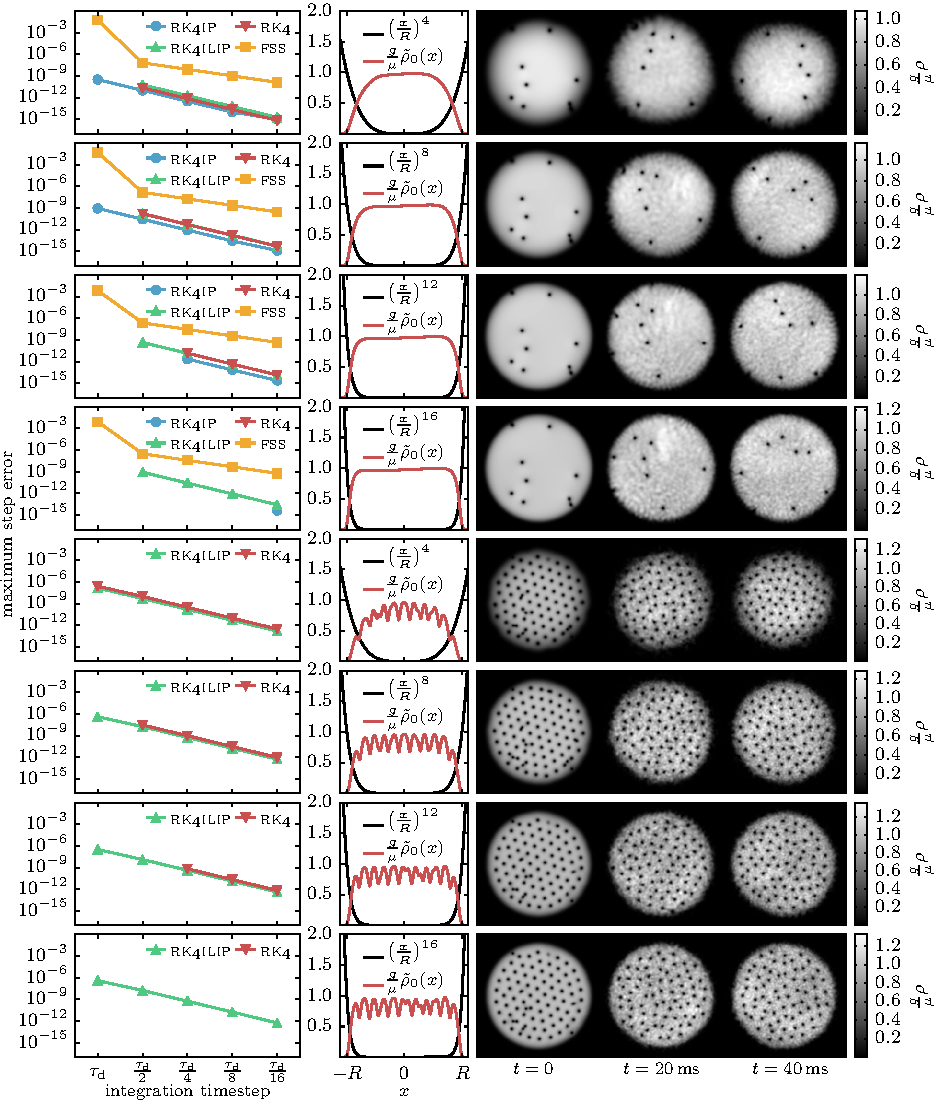
\includegraphics{figures/numerics/rk4ilip_results.pdf}
        \caption{Results of simulations to compare \textsc{rl4ilip} to other timestepping methods.
        Top four rows: Nonrotating frame simulations with four different radial power-law potentials.
        Bottom four rows: Rotating frame simulations with same four potentials.
        Left column: maximum per-step error $\int \abs{\psi - \tilde\psi}^2\,\dd \vec{r}/\int\abs{\tilde\psi}^2\,\dd \vec{r}$ of fourth order Runge--Kutta (\textsc{rk4}), its interaction picture variants (\textsc{rk4ip} and \textsc{rk4ilip}) and Fourier split-step (\textsc{fss}) as a function of timestep. Solutions were checked every $100$ timesteps against a comparison solution $\tilde \psi$ computed using half sized steps for \textsc{rk4} methods, and quarter sized steps for \textsc{fss}. Simulations encountering numerical overflow not plotted.
        Centre column: potential (black) and average density $\tilde \rho_0$ of the initial state  (red) over a slice of width $R/5$ in the $y$ direction.
        Right column: Density of solution at initial, intermediate and final times for each configuration simulated (taken from \textsc{rk4ilip} results).
        \textsc{rk4ilip} is the only method usable in rotating frames and not encountering overflow in the steeper traps for the timesteps considered.}
        \label{fig:rk4ilip_results}
    \end{figure}
    \restoregeometry
}

 Here I compare four numerical methods: Fourier split-step (\textsc{fss}), fourth order Runge--Kutta in the interaction picture (\textsc{rk4ip}), ordinary fourth order Runge--Kutta (\textsc{rk4}), and my new method --- fourth order Runge--Kutta in an instananeous local interaction picture (\textsc{rk4ilip}).

 The example chosen is a \textsc{2d} simulation of a turbulent Bose--Einstein condensate, in both a rotating and nonrotating frame. For the nonrotating frame the differential equation simulated was equation \eqref{eq:RK4_ILIP_GPE}, and for the rotating frame the same equation was with an additional two terms added to the Hamiltonian:
\begin{align}
\hat H_\up{rot} + \hat H_\up {comp} &= -\vec \Omega \cdot \hat{\vec L} +\frac12\hbar m^2\Omega^2 r^2\\
                &= \ii\hbar\Omega \left(x\pdv{y} - y\pdv{x}\right) +\frac12\hbar m^2\Omega^2 r^2.
\end{align}
The addition of the first term transforms the original Hamiltonian into a frame rotating at angular frequency $\Omega$ in the $(x, y)$ plane, and is equivalent to the the Coriolis and centrifugal forces that appear in rotating frames in classical mechanics \cite{Gulshani1978}. The second term is a harmonic potential that exactly compensates for the centrifugal part of this force. In this way the only potential in the rotating frame is the applied trapping potential, and the only effect of the rotating frame is to add the Coriolis force.

 Four trapping potentials were used, all radial power laws with different powers. These examples were chosen to demonstrate the specific situation in which \textsc{rk4ilip} provides a benefit over the other methods for spatial Schr\"odinger-like equations, as discussed above.

The results of $120$ simulation runs are shown in \figref{fig:rk4ilip_results}. Each simulation was of a $\ ^\up{87}$Rb condensate in the $\ket{F=2, m_F=2}$ state, in which the two-body $s$-wave scattering length is $a = 98.98$ Bohr radii \cite{vanKempen2002}. The simulation region was $20\unit{\mu m}$ in the $x$ and $y$ directions, and the Thomas--Fermi radius of the condensate was $R = 9\unit{\mu m}$.  The chemical potential was $\mu = 2\pi\hbar\times 1.91\unit{kHz}$, which is equivalent to a maximum Thomas--Fermi density $\rho_\up{max} = 2.5\E{14}\unit{cm}^{-3}$ and a healing length $\xi = 1.1\unit{\mu m}$. There were $256$ simulation grid points in each spatial dimension, which is $14$ points per healing length.

Four different potentials were used, all of the form $V(r) = \mu \left(r/R\right)^\alpha$ with $\alpha = 4, 8, 12, 16$. For the rotating frame simulations, the rotation frequency was $\Omega = 2\pi \times 148\unit{Hz}$. This is $89\%$ of the effective harmonic trap frequency, defined as the frequency of a harmonic trap that would have the same Thomas--Fermi radius given the same chemical potential.

All ground states were determined using successive over-relaxation (See section [TODO]) with sixth-order finite differences for spatial derivatives. For the nonrotating simulations, convergence was reached with $\upDelta\mu/\mu < 1\E{-13}$, with:
\begin{equation}
\upDelta\mu = \sqrt{\frac{\matrixel{\psi} {(\hat H - \mu)^2}{\psi}}{\braket {\psi}{\psi}}},
\end{equation}
where $\hat H$ is the nonlinear Hamiltonian and $\braket{\vec r}{\psi}$ is the condensate wavefunction, which does not have unit norm. For the rotating frame simulations the ground states converged to $\upDelta\mu/\mu \approx 9\E{-7}, 2\E{-6}, 3\E{-6}$ and $2\E{-6}$ for $\alpha = 16, 12, 8$, and $4$ respectively.

After each ground state was found, it was multiplied by a spatially varying phase factor corresponding to the phase pattern of a number of randomly positioned vortices:
\begin{align}
\psi_\up{vortices}(x, y) = \psi_\up{ground state}(x, y)\prod_{n=1}^N e^{\pm_n i\arctantwo(y - y_n, x - x_n)}
\end{align}
where $\arctantwo$ is the two-argument $\arctan$ function,\footnote{Defined as the principle value of the argument of the complex number $x + iy$: \mbox{$\arctantwo(y, x) = \Arg(x + iy)$.}} $N=30$, $\pm_n$ is a randomly chosen sign, and $(x_n, y_n)$ are vortex positions randomly drawn from a Gaussian distribution centred on $(0,0)$ with standard deviation equal to the Thomas--Fermi radius $R$. The same seed was used for the pseudorandom number generator in each simulation run, and so the vortex positions were identical in each simulation run.

After vortex phase imprinting, the wavefunctions were evolved in imaginary time \cite{chiofalo2000}. For the nonrotating frame simulations, imaginary time evolution was performed for a time interval equal to the chemical potential timescale $\tau_\mu= 2\pi\hbar/\mu$, and for the rotating frame simulations, for $\tau_\mu/10$. This was done to smooth out the condensate density in the vicinity of vortices, producing the correct density profile for vortex cores. However, since imaginary time evolution decreases the energy of the state indiscriminately, it also had the side effect of causing vortices of opposite sign to move closer together and annihilate. This decreased the number of vortices, and is the reason the smoothing step in the rotating frame simulations was cut short to $\tau_\mu/10$, as otherwise all vortices had time to annihilate with one of the lattice vortices. A vortex pair in the process of annihilating is visible in \figref{fig:rk4ilip_results} as a partially filled hole in the initial density profile near the top of the condensate in the $\alpha=4, 12,$ and $16$ rotating frame simulations.\footnote{The initial states for the four different potentials are not identical, so by chance the corresponding vortex in the $\alpha=8$ case was not close enough to a lattice vortex to annihilate.}

The smoothed, vortex imprinted states were then evolved in time for $40\unit{ms}$. For each simulation, five different timesteps were used: $\upDelta t = \tau_\up d, \tau_\up d / 2, \tau_\up d / 4, \tau_\up d / 8, \tau_\up d / 16$, where \mbox{$\tau_\up d = m \upDelta x^2 / \pi\hbar \approx 2.68\unit{\mu s}$} is the dispersion timescale associated with the grid spacing $\upDelta x$, defined as the time taken to move one gridpoint at the group velocity of the Nyquist mode.

For the nonrotating frame simulations, spatial derivatives for the \textsc{rk4} and \textsc{rk4ilip} methods were determined using the Fourier method [see section TODO]. This was to ensure a fair comparison with the other two methods, which necessarily use Fourier transforms to perform computations pertaining due to the kinetic term.

For the rotating frame simulations, sixth-order finite differences with zero boundary conditions were used instead for the kinetic terms of the \textsc{rk4} and \textsc{rk4ilip} methods, which were the only two methods used for those simulations (due to the other methods being incompatible with the angular momentum operator required for a rotating frame). This choice was fairly arbitrary, but did allow the condensate to be closer to the boundary than is otherwise possible with the periodic boundary conditions imposed by use of the Fourier method for spatial derivatives. This is because the rotating frame Hamiltonian is not periodic in space, and so its discontinuity at the boundary can be a problem if the wavefunction is not sufficiently small there.

As shown in \figref{fig:rk4ilip_results}, all methods tested generally worked well until they didn't work at all, with the per-step error of \textsc{rk4}-based methods being either small and broadly the same as the other \textsc{rk4}-based methods, or growing rapidly to the point of numerical overflow (shown as missing datapoints). The break down of \textsc{fss} was less dramatic, though it too had a clear jump in its per-step error for larger timesteps. Comparing methods therefore came down to mostly whether or not a simulation experienced numerical overflow during the time interval being simulated.

The main result was that \textsc{rk4ilip} and \textsc{fss} remained accurate over the widest range of timesteps and trap steepnesses, with \textsc{rk4} and \textsc{rk4ip} requiring ever smaller timesteps in order to not overflow as the trap steepness increased.

For the rotating frame simulations, which were only amenable to the \textsc{rk4} and \textsc{rk4ilip} methods, the same pattern was observed, with \textsc{rk4} only working at smaller timesteps as the trap steepness was increased, and ultimately diverging for all timesteps tested at the maximum trap steepness. By contrast, \textsc{rk4ilip} remained accurate over the entire range of timesteps at the maximum trap steepness.

\subsection{Discussion}

As mentioned, \textsc{rk4ilip} is mostly useful for continuum quantum mechanics only when there are large spatial differences in the potential, which cannot give rise to equally large kinetic energies\footnote{This is essentially due to such a situation violating the condition we laid out at the beginning of this section --- that the simulation basis must be nearly an eigenbasis of the total Hamiltonian.}. Furthermore, the advantage that \textsc{rk4ilip} has over other methods with that same property is that it is does not require a particular form of Hamiltonian or a particular method of evaluating spatial derivatives. The former means is is applicable in rotating frames or to situations with unusual Hamiltonians, and the latter means is can be used with finite differences or \textsc{fedvr} \cite{schneider_parallel_2006} and thus is amenable to parallelisation on a cluster computer.

The ability to model large spatial variations in the potential provides only a narrow domain of increased usefulness over other methods. If a large kinetic energy results from the large potential, then the method requires just as small timesteps as any other. And if the large potential is supposed to approximate an an infinite well, then an actual infinite well may be modelled using zero boundary conditions, negating the need for something like \textsc{rk4ilip}. However, when potential wells are steep, but not infinitely steep, here \textsc{rk4ilip} provides a benefit. The only other model that can handle these large potentials---Fourier split-step---has the disadvantage that it cannot deal with arbitrary operators such as those arising from a rotating frame, and is not parallelisable with local data. The benefits of parallelisability are obvious, and the above results demonstrate \textsc{rk4ilip}'s advantage at simulating \textsc{bec}s in tight traps and rotating frames.

Note that whilst the \emph{Fourier} split-step method can't handle Hamiltonian terms such as $\hat {\vec r} \cdot \hat {\vec p}$ that are not diagonal in either real space or Fourier space \cite[p315]{tannor_introduction_2007}, a split-step method based on an approximation to the momentum operator as a banded matrix, such as that obtained with finite differences, can. Using the techniques discussed in section \ref{sec:split-step-parallel}, such a scheme is also parallelisable. The remaining limitations then, when compared to fourth-order Runge--Kutta are the restriction on the types of nonlinearity that can be included, and the complexity of implementation.

For systems with discrete degrees of freedom, \textsc{rk4ilip} may be useful in the case where an approximate diagonalisation of the Hamiltonian is analytically known, and when the Hamiltonian's eigenvalues vary considerably in time (making a single interaction picture insufficient to factor out dynamical phases throughout the entire simulation). In this situation an analytic transformation into the diagonal basis can be performed at each timestep (or the differential equation analytically re-cast in that basis in the first place), and \textsc{rk4ilip} can be used to factor out the time-varying dynamical phase evolution at each timestep. An example may be an atom with a magnetic moment in a time-varying magnetic field which varies over orders of magnitude. The transformation into the spin basis in the direction of the magnetic field can be analytically performed, and if the field varies by orders of magnitude, so do the eigenvalues of the Hamiltonian. Although the eigenvalues in this case and other similar cases can be computed analytically too, unless all time dependence of the Hamiltonian is known in advance of the simulation, it would be difficult to incorporate this into a re-casting of the differential equation in a time-dependent interaction picture. \textsc{rk4ilip} may be useful in these cases to automate this process and evolve the system in the appropriate interaction picture at each timestep.
